\chapter{System Design and Architecture}

\section{Introduction}
This chapter details the design and architecture of the robotic sorting cell. It provides a technological overview and then focuses on the hardware and software architecture, covering the selection and integration of all operative and control components, such as the KUKA robot, conveyors, sensors, and the control cabinets.

\section{Technological Overview}
Automated sorting is a fundamental application of industrial automation, critical for increasing efficiency, consistency, and speed in various sectors, including logistics, food processing, and recycling. Modern sorting systems integrate technologies such as vision systems, industrial robots, and PLC-based control systems to classify and handle objects.

The design of this project was informed by similar systems that showcase the effective combination of vision, robotics, and automation for sorting tasks. Examples of such systems are provided below:

\begin{itemize}
    \item \textbf{FANUC M‑1iA – Pill Sorting Cell}: This high-speed sorting cell uses a FANUC M-1iA robot with an iRVision system to classify small objects by color \cite{FANUC}\hyperref[sec:bibliography]{[3]}. The cell is shown in Figure \ref{fig:FANUC_PillSorting}.
    \begin{figure}[H]
        \centering
        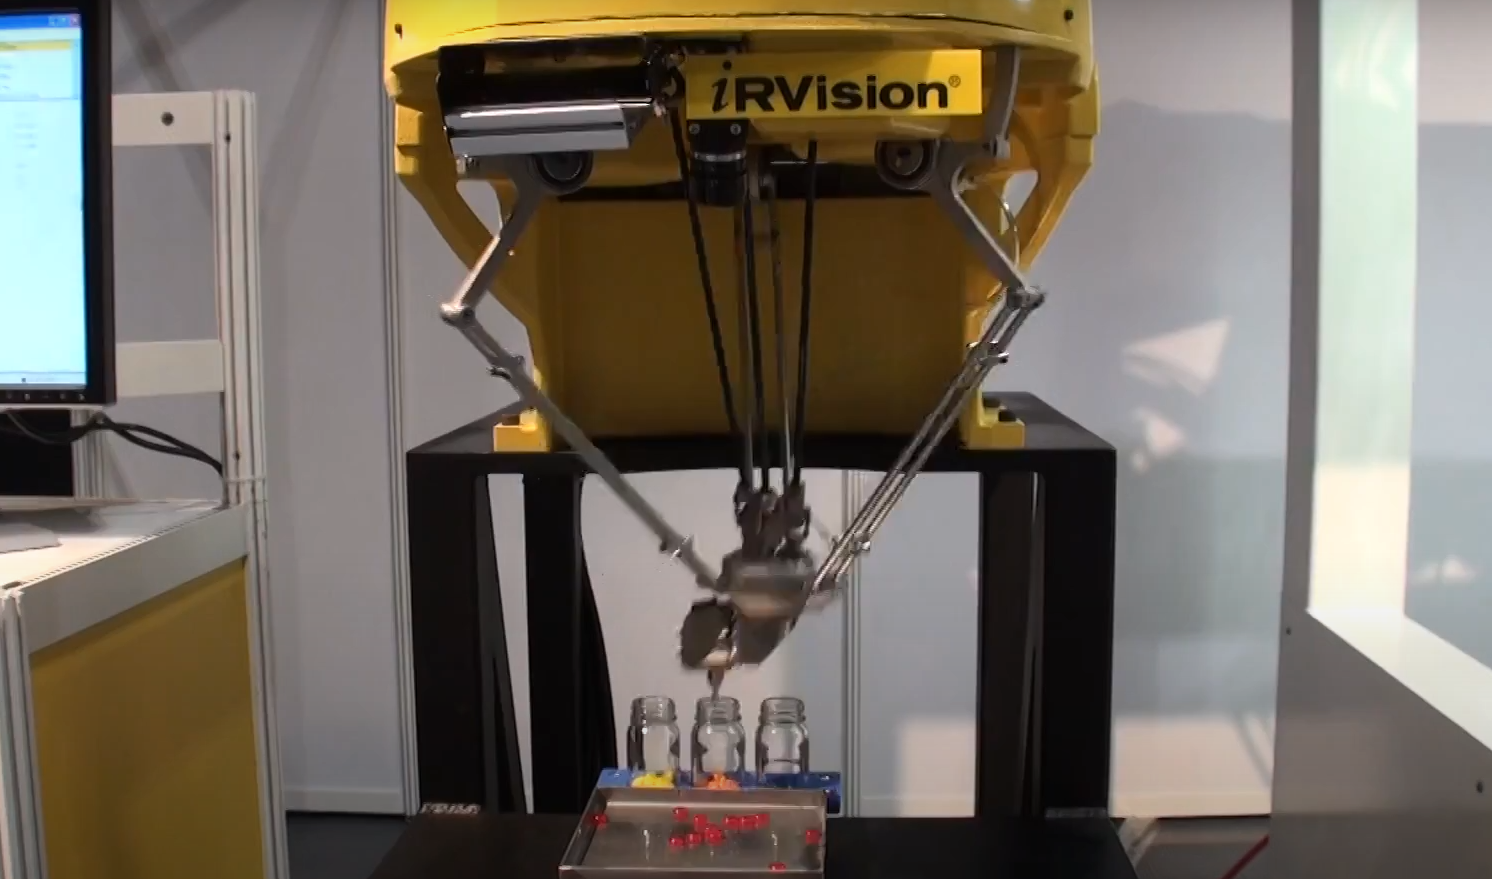
\includegraphics[width=0.8\textwidth]{Images/Chap2/FANUC.png}
        \caption[FANUC M‑1iA – Pill Sorting Demonstration Cell]{FANUC M‑1iA – Pill Sorting Demonstration Cell}
        \label{fig:FANUC_PillSorting}
    \end{figure}
    \item \textbf{ABB IRB 360 – Snack Sorting and Packaging Cell}: An ABB IRB 360 robot with a PickMaster vision system sorts and packages snacks at high speed, demonstrating a food packaging application \cite{ABB}\hyperref[sec:bibliography]{[4]}. The cell is illustrated in Figure \ref{fig:ABB_SnackSorting}.
   \begin{figure}[H]
    \centering
    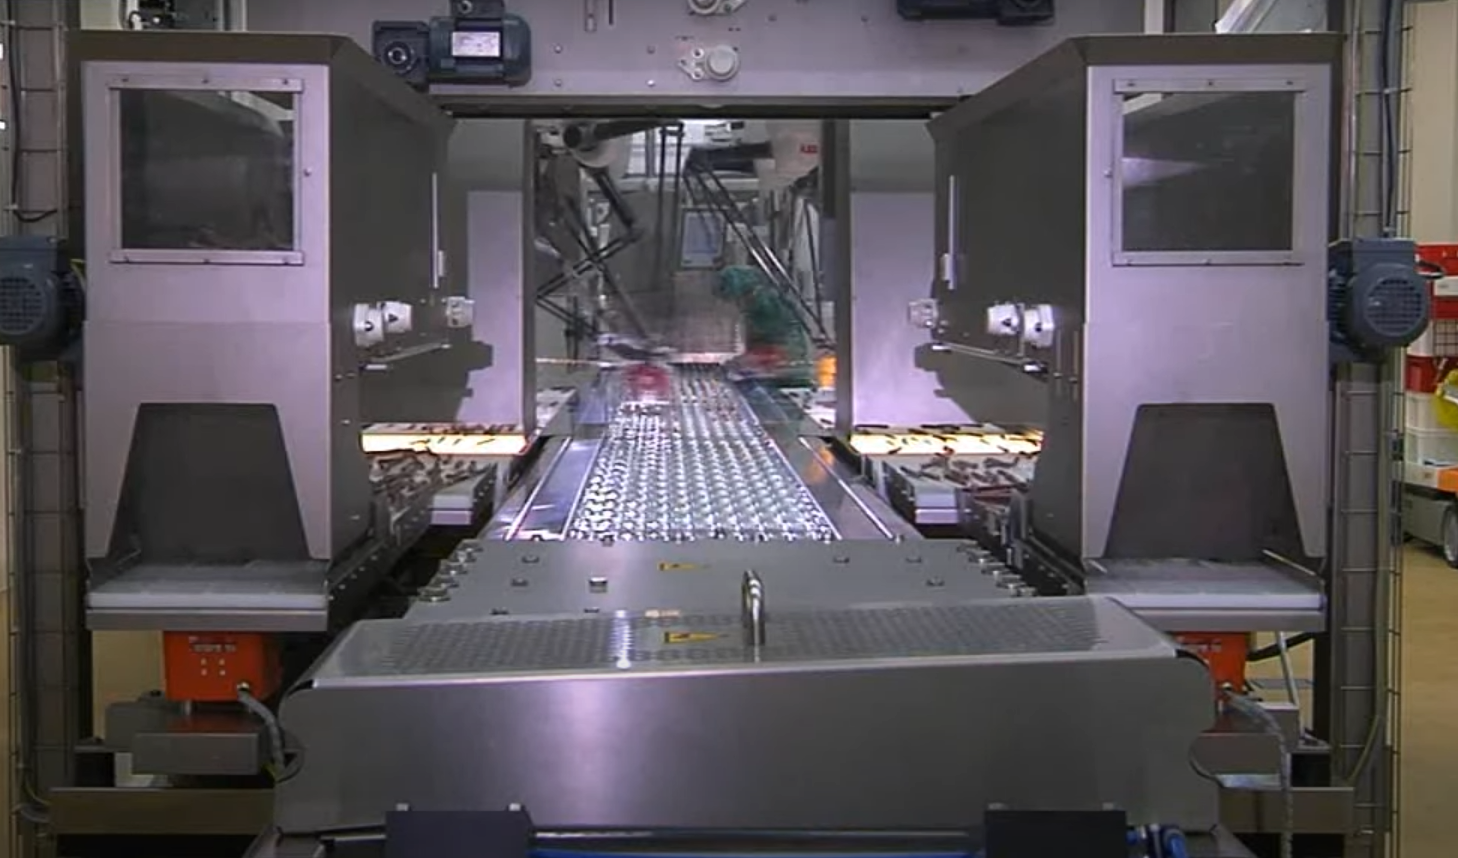
\includegraphics[width=0.45\textwidth]{Images/Chap2/ABB1.png}
    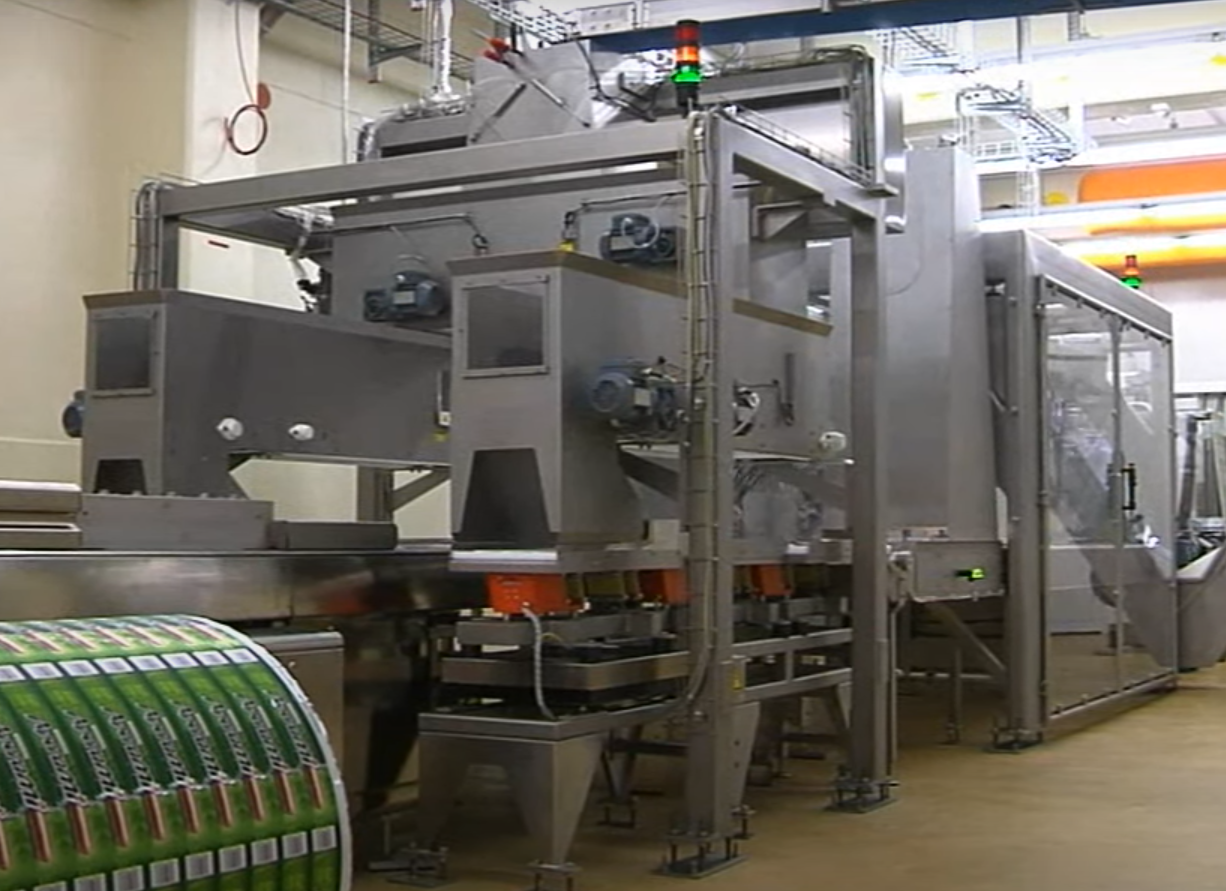
\includegraphics[width=0.45\textwidth]{Images/Chap2/ABB2.png}
    \caption[ABB IRB 360 – Snack Sorting and Packaging Cell]{ABB IRB 360 – Snack Sorting and Packaging Cell}
    \label{fig:ABB_SnackSorting}
\end{figure}
    \item \textbf{ZenRobotics Recycler – Waste Sorting Cell}: This autonomous waste sorting system combines robotic arms, cameras, and AI to separate materials like metal and plastic from construction waste, processing up to 3000 objects per hour \cite{ZenRobotics}\hyperref[sec:bibliography]{[5]}. An example of this system is shown in Figure \ref{fig:ZenRobotics_WasteSorting}.
    \begin{figure}[H]
        \centering
        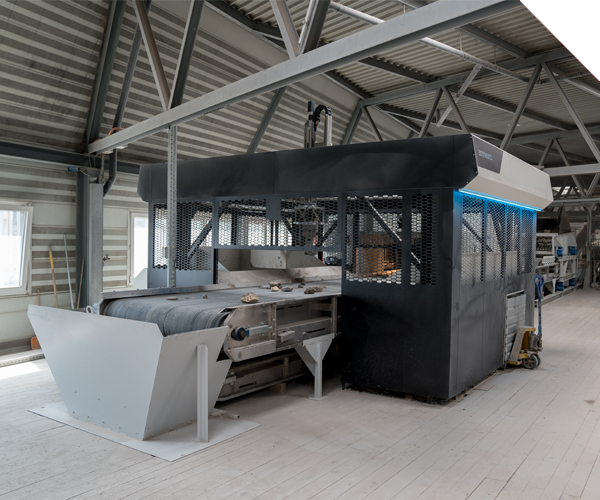
\includegraphics[width=0.6\textwidth]{Images/Chap2/ZenRobotics.png}
        \caption[ZenRobotics Recycler – Waste Sorting Cell]{ZenRobotics Recycler – Waste Sorting Cell}
        \label{fig:ZenRobotics_WasteSorting}
    \end{figure}
\end{itemize}

\section{Hardware Architecture}
The hardware architecture encompasses all physical components, including the operative part (sensors and actuators), the control part (PLC, HMI, robot controller), and supporting systems.

\subsection{Operative Part}
This part consists of the physical elements that interact directly with the environment, including actuators and sensors.

\subsubsection{Actuators}
\begin{itemize}
  \item \textbf{KUKA Robot - KR AGILUS}: The six-axis KUKA KR AGILUS robot was chosen as the main manipulator due to its compact size, high speed, and exceptional repeatability of $\pm0.03$ mm. It is controlled by a KRC4 Compact controller that communicates with the PLC via industrial Ethernet. The robot's technical specifications are detailed in Table \ref{tab:kuka_specs}. A visual representation of the robot is provided in Annex \ref{fig:KukaRobot}, and its six-axis configuration is shown in Annex \ref{fig:KukaAxis}.
    \renewcommand{\arraystretch}{1.3} 
    \begin{table}[H] 
    \centering 
    \caption{Technical Specifications of the KR AGILUS Robot} 
    \label{tab:kuka_specs} 
    \begin{tabularx}{\textwidth}{|l|X|} 
     \hline 
     \textbf{Parameter} & \textbf{Value} \\ 
     \hline 
     Model & KR 6 R700 (AGILUS series) \\ 
     \hline 
     Degrees of Freedom & 6 axes \\ 
     \hline 
     Maximum Payload & 6 kg \\ 
     \hline 
     Reach & 706.7 mm \\ 
     \hline 
     Repeatability & $\pm0.03$ mm \\ 
     \hline 
     Controller & KRC4 Compact \\ 
     \hline 
     Protection Rating & IP54 \\ 
     \hline 
     Mounting Positions & Floor, ceiling, wall \\ 
     \hline 
    \end{tabularx} 
    \end{table}
    

    
    \item \textbf{Belt Conveyors}: Two perpendicular Dierre belt conveyors create a compact L-shaped flow for transporting colored cubes. Each is powered by an SMT 5634 geared motor and controlled by the PLC to operate at a fixed speed. The main specifications are listed in Table \ref{tab:conveyor_specs}. The conveyor belt used in the cell is shown in Figure \ref{fig:conveyor_real}.
    
    \renewcommand{\arraystretch}{1.3}
    \setlength{\tabcolsep}{10pt}
    
    \begin{table}[H]
        \centering
        \caption{Technical Specifications of the Conveyor System}
        \label{tab:conveyor_specs}
        \begin{tabularx}{\textwidth}{|l|X|}
            \hline
            \textbf{Parameter} & \textbf{Value} \\
            \hline
            Manufacturer & Dierre \\
            \hline
            Motor & SMT 5634 \\
            \hline
            Control Method & PLC-controlled contactor \\
            \hline
            Speed & Fixed \\
            \hline
            Dimensions & Approx. 1000 mm length / 150 mm width \\
            \hline
        \end{tabularx}
    \end{table}

    \begin{figure}[H]
        \centering
        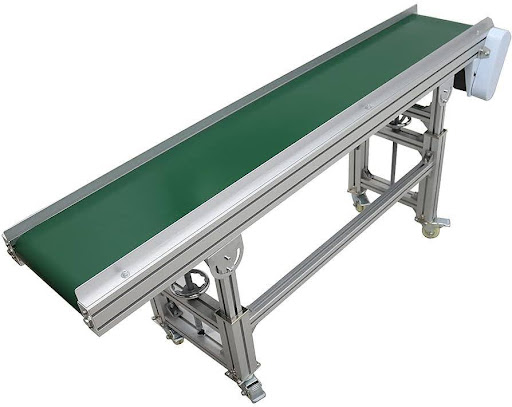
\includegraphics[width=0.35\textwidth]{Images/Chap2/Conveyor.jpg}
        \caption[Conveyor Belt Used in the Sorting Cell]{Dierre conveyor belt used for part transport}
        \label{fig:conveyor_real}
    \end{figure}

    \item \textbf{Pneumatic Cylinders}: Two Festo guided cylinders were integrated for precise, stable linear motion to push cubes into position. Their compact design was ideal for the limited space. An example of the cylinder used is shown in Figure \ref{fig:Festo_Cylinder}.
    \begin{figure}[H]
        \centering
        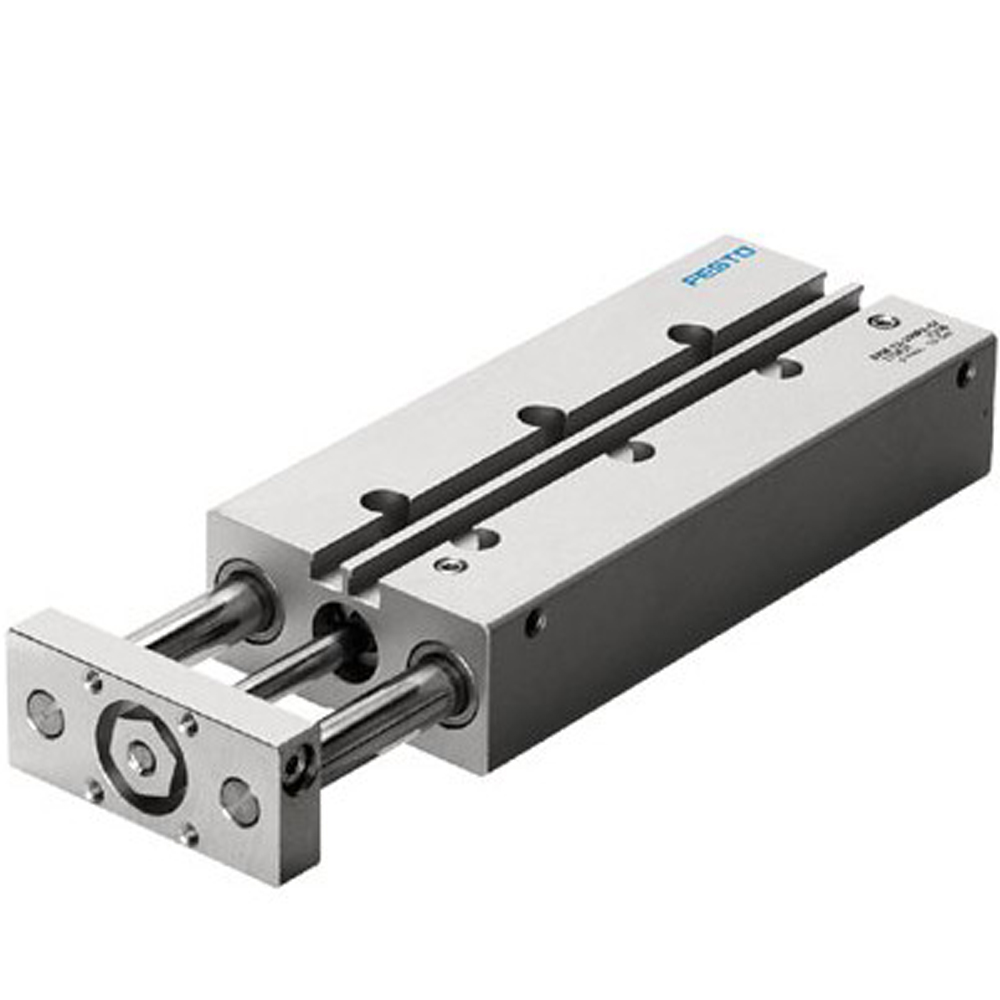
\includegraphics[width=0.32\textwidth]{Images/Chap2/verin.jpg}
        \caption[Festo Guided Pneumatic Cylinder]{Festo Guided Pneumatic Cylinder}
        \label{fig:Festo_Cylinder}
    \end{figure}

    \item \textbf{Prehenseur (Gripper)}: A custom-designed pneumatic parallel jaw gripper, specifically a Festo type, was developed as the robot's end-effector. This device uses a pneumatic cylinder to provide the gripping force and is sized to securely handle the colored cubes. The gripper is shown in Figure \ref{fig:gripper}.
    \begin{figure}[H]
        \centering
        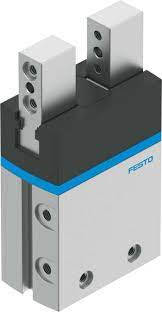
\includegraphics[width=0.18\textwidth]{Images/Chap2/gripper.jpg}
        \caption[Pneumatic Parallel Jaw Gripper]{Pneumatic Parallel Jaw Gripper}
        \label{fig:gripper}
    \end{figure}
\end{itemize}

\subsubsection{Sensors}
In the designed sorting cell, a set of sensors was integrated to enable real-time feedback and ensure accurate synchronization between the different automated components, including conveyors, pneumatic actuators, and the robot. These sensors play a critical role in detecting the presence of objects, confirming part positions, and triggering control events within the PLC logic.

\begin{itemize}
    \item \textbf{OMRON E3Z-D61 2M}:
    Two OMRON E3Z-D61 photoelectric sensors were integrated into the sorting cell to detect the presence of cubes during critical stages of the process. One sensor was placed in front of the guided cylinder, between the two conveyors, and the other in front of the vision system camera. These sensors were chosen for their compact size, diffuse detection capability, and reliable performance with colored plastic objects under varying ambient lighting.
    The main characteristics and functions of the installed sensors are summarized in Table \ref{tab:omron_specs}. A visual representation of the sensor is shown in Figure \ref{fig:Omron_Sensor}.
    \renewcommand{\arraystretch}{1.3}
    \setlength{\tabcolsep}{10pt}
    
    \begin{table}[H]
        \centering
        \caption{OMRON E3Z-D61 Sensor Specifications}
        \label{tab:omron_specs}
        \begin{tabularx}{\textwidth}{|l|X|}
            \hline
            \textbf{Parameter} & \textbf{Value} \\
            \hline
            Sensing method & Diffuse reflective \\
            \hline
            Sensing distance & 100 mm \\
            \hline
            Min sensing distance & 5 mm \\
            \hline
            Response time & 1 ms \\
            \hline
            Width & 10.8 mm \\
            \hline
            Height & 31 mm \\
            \hline
            Depth & 20 mm \\
            \hline
            Type of light & Infrared light \\
            \hline
            Power supply voltage & 12-24 V \\
            \hline
        \end{tabularx}
    \end{table}

    \begin{figure}[H]
        \centering
        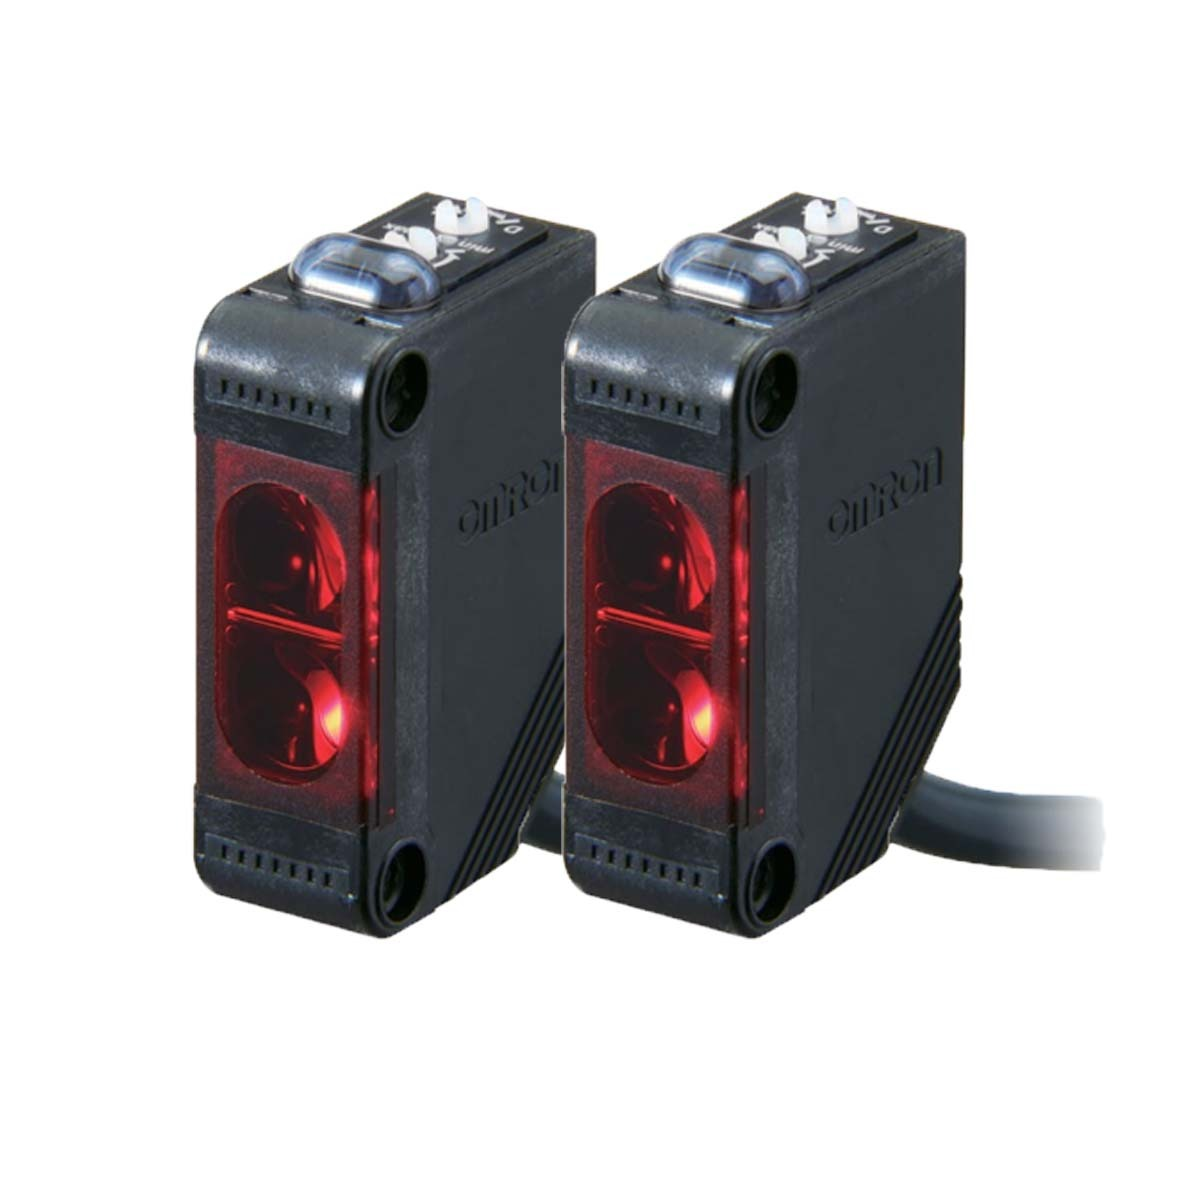
\includegraphics[width=0.4\textwidth]{Images/Chap2/OmronSensor.jpg}
        \caption[OMRON E3Z-D61 Sensor]{OMRON E3Z-D61 Sensor}
        \label{fig:Omron_Sensor}
    \end{figure}

    \item \textbf{Proximity Sensors for Cylinders (FESTO SMT-8M-A-PS-24V-E-0,3-M8D)}
    
    To ensure accurate control and positioning of the pneumatic actuators, Festo SMT-8M-A-PS-24V-E-0,3-M8D proximity sensors were installed on each cylinder. These sensors detect the piston’s position and provide feedback to the PLC, allowing precise monitoring of the extension and retraction states.
    A total of five sensors were used across the system. Two sensors were mounted on each of the two main guided cylinders to detect both end positions. The remaining sensor was placed on the final storage-area cylinder, where only the fully extended position needed to be confirmed. This configuration ensures that the system always has reliable information on whether a part has been moved, aligned, or stored correctly.
    
    These magnetic proximity sensors offer non-contact detection, resulting in long service life, resistance to mechanical wear, and quick response time. Their compact format and easy mounting grooves make them ideal for cylinder-based installations. The sensors were directly wired to the PLC's digital input terminals, enabling real-time logic decisions within the automation sequence.
    
    The technical specifications of the sensors are summarized in Table \ref{tab:festo_proximity_specs}. A visual representation of the sensor is provided in Figure \ref{fig:Festo_Proximity_Sensor}.
    \renewcommand{\arraystretch}{1.3}
    \setlength{\tabcolsep}{10pt}
    \begin{table}[H]
        \centering
        \caption{Technical Specifications of the Festo Cylinder Proximity Sensors}
        \label{tab:festo_proximity_specs}
        \begin{tabularx}{\textwidth}{|l|X|}
            \hline
            \textbf{Parameter} & \textbf{Value} \\
            \hline
            Manufacturer & Festo \\
            \hline
            Type & Magnetic proximity sensor for pneumatic cylinders \\
            \hline
            Quantity & 5 (2 per cylinder on main axes, 1 for storage cylinder) \\
            \hline
            Detection Type & Magnetic field detection (non-contact) \\
            \hline
            Application & Detect end-of-stroke positions of pneumatic actuators \\
            \hline
            Mounting & Integrated groove on cylinder body \\
            \hline
            Connection Type & Cable with connector to PLC input \\
            \hline
            Response Time & Switch-on time : < 1.3 ms / Switch-off time : < 7.3 ms \\
            \hline
            Advantages & Long service life, wear-free, compact, easy installation \\
            \hline
            Operational voltage range DC & 5 V ... 30 V \\
            \hline
        \end{tabularx}
    \end{table}
    \begin{figure}[H]
        \centering
        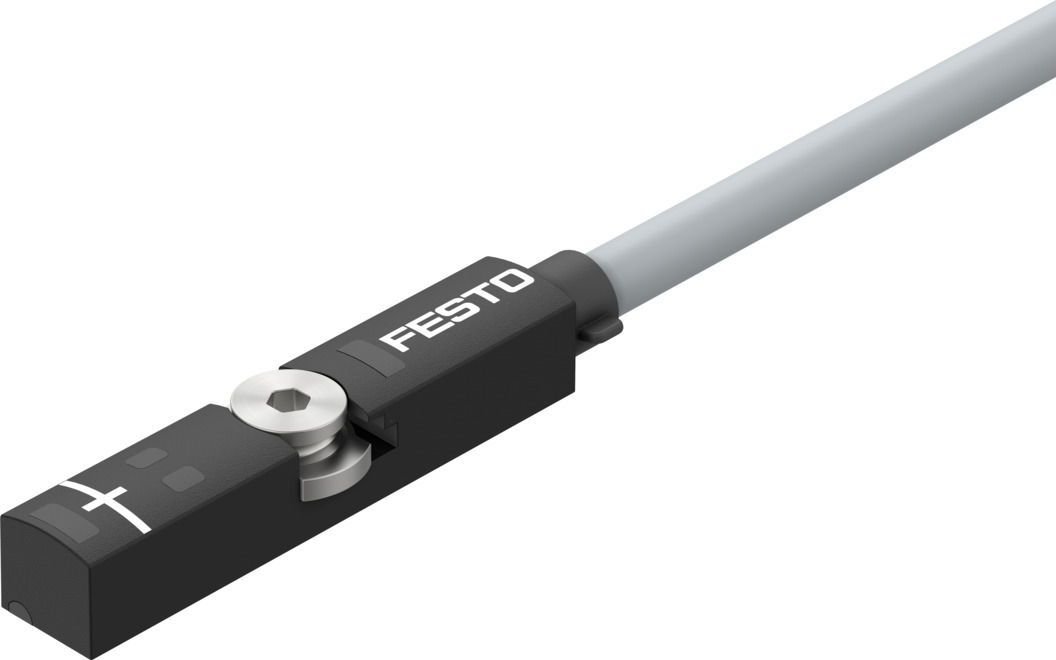
\includegraphics[width=0.35\textwidth]{Images/Chap2/proximetsensor.jpg}
        \caption[ Festo Proximity Sensors for Cylinders ]{Festo Proximity Sensors for Cylinders}
        \label{fig:Festo_Proximity_Sensor}
    \end{figure}
\end{itemize}





\subsection{Control Part}
The control part includes all the components responsible for managing and coordinating the actions of the automated system. It interprets sensor data, executes logical decisions, and generates appropriate commands to drive actuators. This part typically consists of programmable logic controllers (PLCs), human-machine interfaces (HMIs), and communication modules. Together, these elements ensure that the system operates safely, efficiently, and in accordance with predefined sequences.

\begin{itemize}
    \item \textbf{Programmable Logic Controller (PLC)}:

    The programmable logic controller (PLC) is the core of the control system. It processes sensor inputs, executes the automation logic, and drives the actuators accordingly. In this project, the PLC is responsible for managing the entire sorting cycle, including cylinder control, conveyor coordination, sensor supervision, and real-time interaction with the HMI and external devices such as the industrial robot and Raspberry Pi. A digital-only I/O configuration was required, and network-based communication played a key role in the component selection process.


    The selection of the programmable logic controller (PLC) was based on key functional requirements derived from the automation and communication needs of the sorting cell. These requirements included:
    
    -At least 11 digital inputs (e.g., sensors, endstops, Buttons)
    
    -At least 11 digital outputs (e.g., solenoid valves, conveyor motors, Lights)
    
    -Three Ethernet connections (Robot controller, Raspberry Pi, HMI)

    The selected PLC had to support Siemens' TIA Portal ecosystem and provide expansion flexibility while keeping the total cost within a reasonable budget. Two possible configurations from different Siemens product families were considered and compared based on their I/O capacity, communication features, and overall cost, as shown in Table \ref{tab:plc_siemens_comparison}.
    \renewcommand{\arraystretch}{1.3}
    \setlength{\tabcolsep}{8pt}

    \begin{table}[H]
        \centering
        \caption{Comparison of Siemens PLC Configurations}
        \label{tab:plc_siemens_comparison}
        \begin{tabularx}{\textwidth}{|l|X|X|X|X|}
            \hline
            \textbf{Solution} & \textbf{PLC Family and Modules} & \textbf{I/O Capacity} & \textbf{Ethernet Support} & \textbf{Estimated Cost (€)} \\
            \hline
            \textbf{A} & \textbf{S7-1212C} + SB module + Ethernet switch & 14 DI / 10 DO + 4 DI / 2 DO & 1 (add switch to split) & ~350 € \\
            \hline
            \textbf{C} & \textbf{S7-1500 (CPU 1511)} + SM1223 module & 14 DI / 10 DO + 8 DI / DO & 2 native ports + Profinet & ~650 € \\
            \hline
        \end{tabularx}
    \end{table}

    After evaluating the available options, Solution A, based on the S7-1212C from the S7-1200 series, was selected. This choice provided a good balance between I/O capacity, communication flexibility, and cost. The Siemens S7-1212C is shown in Figure \ref{fig:siemens_plc}.

    Although the base CPU only includes one Ethernet port, a standard industrial Ethernet switch was added to fulfill the requirement for three simultaneous Ethernet connections. The input/output capacity was covered using a compact signal board (SB), and the option for additional expansion modules remains available if future needs arise.

    This solution ensured full integration with the Siemens TIA Portal environment, supported Profinet communication with the robot and HMI, and kept the system modular and maintainable for demonstration and industrial fair use.

    \begin{figure}[H]
        \centering
        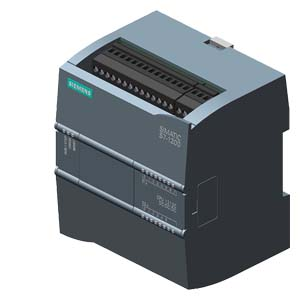
\includegraphics[width=0.3\textwidth]{Images/Chap2/PLC.jpg}
        \caption[Siemens S7-1212C ]{Siemens S7-1212C}
        \label{fig:siemens_plc}
    \end{figure}
    
    \item \textbf{Human-Machine Interface (HMI)}:

    The Human-Machine Interface (HMI) enables system supervision and interaction, providing real-time feedback to the operator regarding the sorting cycle, sensor states, and manual overrides. The selected HMI had to support Siemens' WinCC Unified platform to enable both local touchscreen operation and remote control through a standard web browser, which is particularly useful for demonstration and maintenance purposes during trade fairs. A visual representation of the panel is shown in Figure \ref{fig:tp1200}.

    To satisfy the visualization and usability requirements, a \textbf{12-inch Siemens Unified Comfort Panel} was selected. Specifically, the \textbf{TP1200 Unified} panel was chosen as it offers a high-resolution display, Unified Runtime support, and Profinet communication capabilities at a reasonable cost. Its compatibility with TIA Portal and Unified architecture ensures seamless integration with the control system.

    Additional implementation details regarding screen content and remote access will be addressed in later sections.

    \begin{figure}[H]
        \centering
        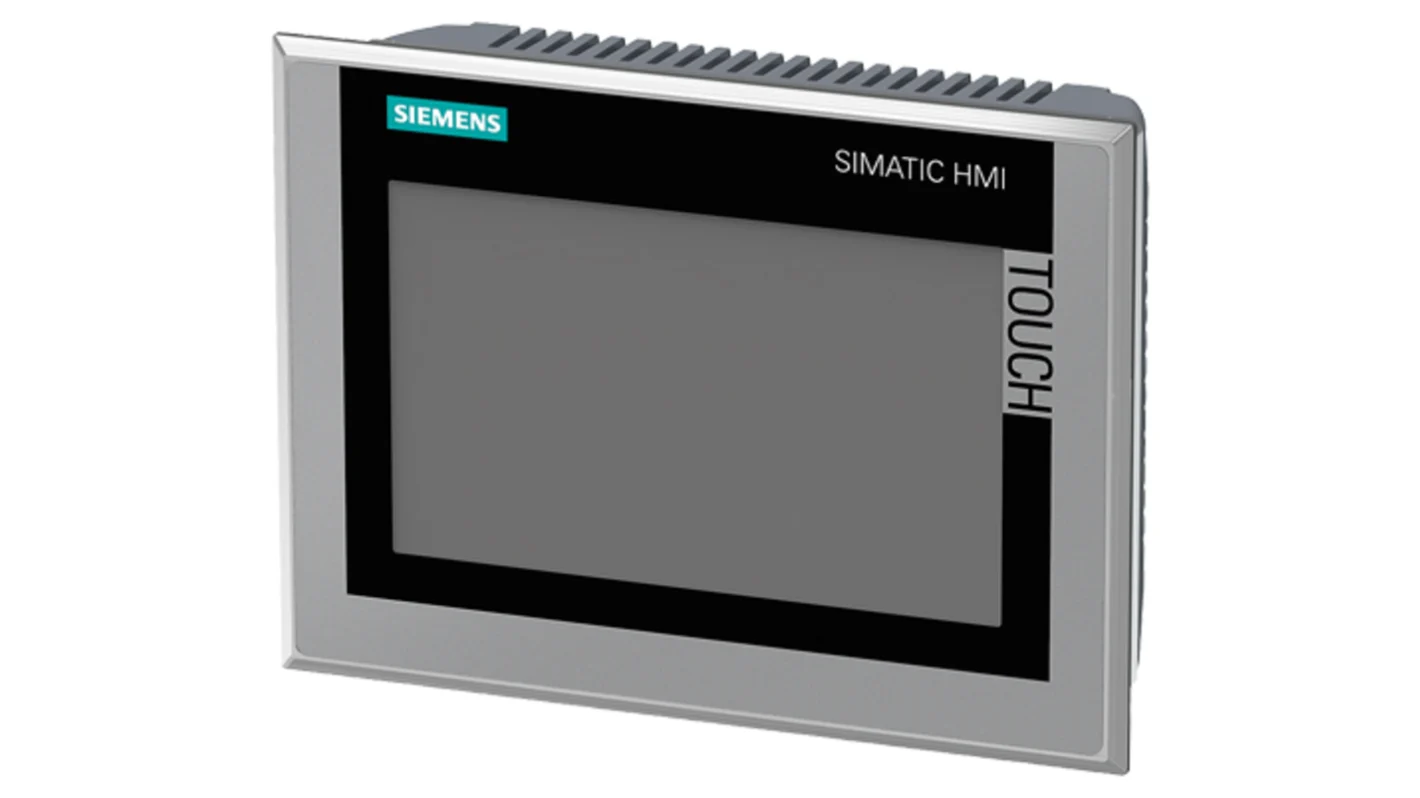
\includegraphics[width=0.5\textwidth]{Images/Chap2/TP1200_Unified.png} % replace with actual path
        \caption[TP1200 Unified Comfort Panel]{TP1200 Unified Comfort Panel (12.1") }
        \label{fig:tp1200}
    \end{figure}
    
    \item \textbf{Robot Controller}:

    The KUKA industrial robot used in this project is managed through a \textbf{KRC4 Compact} controller, which serves as the interface between the robot and the rest of the automation system. This controller handles the motion logic, safety configurations, and communication protocols necessary to integrate the robot into the control architecture. The KRC4 Compact Controller is shown in Figure \ref{fig:krc4compact}.

    The controller is configured using KUKA.WorkVisual software, which allows the setup of I/O mappings and Profinet communication. In this setup, the KRC4 Compact operates as a Profinet device connected to the PLC, allowing synchronization with the overall automation sequence.

    \begin{figure}[H]
        \centering
        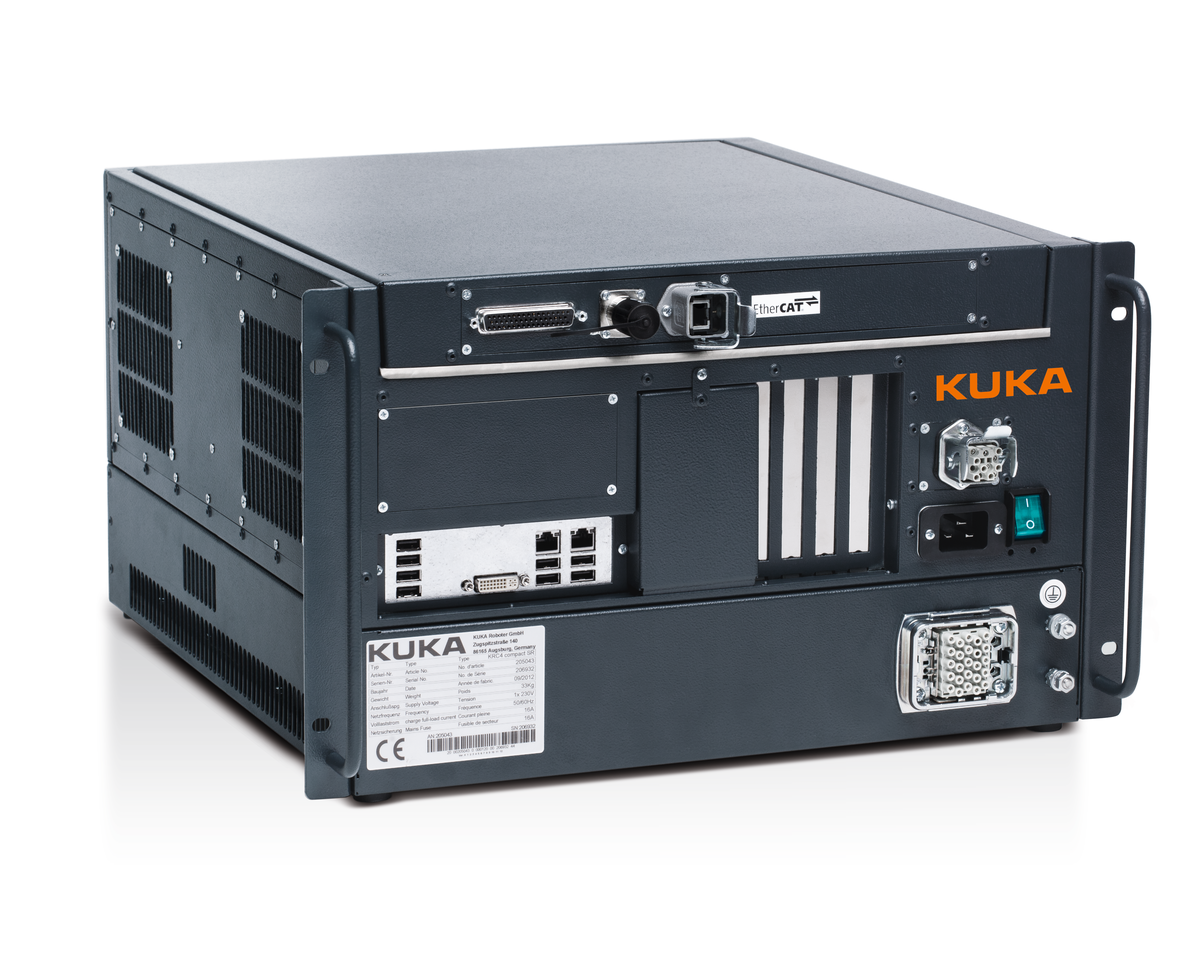
\includegraphics[width=0.45\textwidth]{Images/Chap2/KRC4.png} % replace with actual image
        \caption[KRC4 Compact Controller]{KUKA KRC4 Compact Robot Controller}
        \label{fig:krc4compact}
    \end{figure}

\end{itemize}

\subsection{Electrical Cabinet}
The electrical cabinet serves as the central hub for power distribution, protection, and control within the automated system. All main control components—including the PLC, contactors, power supplies, terminals, and circuit protection devices—are housed inside this enclosure. The cabinet ensures safe and organized wiring, while also facilitating maintenance and future scalability.

\subsubsection{Electrical Wiring Diagram}
To ensure the correct integration and protection of all electrical components, a detailed wiring diagram was created. This diagram represents the overall electrical architecture, including power distribution, component connections, protection devices, and control wiring, and can be seen in Annex \ref{fig:electrical_diagram}.


\subsubsection{Protection components}
This section details the essential components used for circuit protection within the electrical cabinet. These components are vital for safeguarding the entire system against electrical faults, such as overcurrents and short-circuits. By ensuring the integrity of the circuits, they prevent damage to expensive equipment and, more importantly, guarantee the safety of the operating environment. The specific components are outlined in \ref{tab:protection_components}.

\begin{table}[H]
    \centering
    \caption{Protection Components Used in the Electrical Cabinet}
    \label{tab:protection_components}
    \begin{tabularx}{\textwidth}{| >{\raggedright}p{0.3\textwidth} | >{\centering}m{0.2\textwidth} | >{\centering\arraybackslash}m{2.3cm} | X |}
        \hline
        \textbf{Name and Description} & \textbf{Brand} & \textbf{Figure} & \textbf{Function} \\
        \hline
        \textbf{Motor circuit breaker, TeSys GV2, 3P, 4-6.3 A, thermal magnetic, screw clamp terminals} & Schneider Electric &
        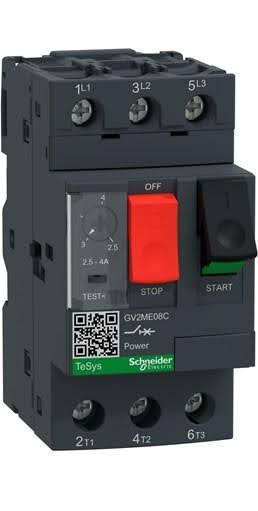
\includegraphics[width=2cm]{Images/Chap2/TeSys GV2.jpg} & Provides overload and short-circuit protection for motor circuits. \\
        \hline
        \textbf{Overcurrent circuit breaker Easy9, 1P+N, 16A, curve C, 4.5kA, type CA, 30mA} & Schneider Electric &
        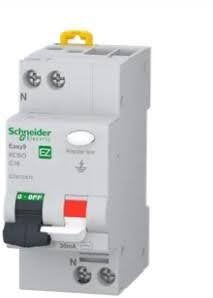
\includegraphics[width=2.2cm]{Images/Chap2/Schneider1.jpg} & Provides overcurrent and differential protection. \\
        \hline
    \end{tabularx}
\end{table}
\subsubsection{Power converters components}
This section outlines the power converter components responsible for providing stable DC power to the system's control elements. These components are listed in Table \ref{tab:power_converter_components}.
\begin{table}[H]
    \centering
    \caption{Power Converter Components Used in the Electrical Cabinet}
    \label{tab:power_converter_components}
    \begin{tabularx}{\textwidth}{| >{\raggedright}p{0.3\textwidth} | >{\centering}m{0.2\textwidth} | >{\centering\arraybackslash}m{2.5cm} | X |}
        \hline
        \textbf{Name and Description} & \textbf{Brand} & \textbf{Figure} & \textbf{Function} \\
        \hline
        \textbf{Power Supply MDR-60-24} & Mean Well &
        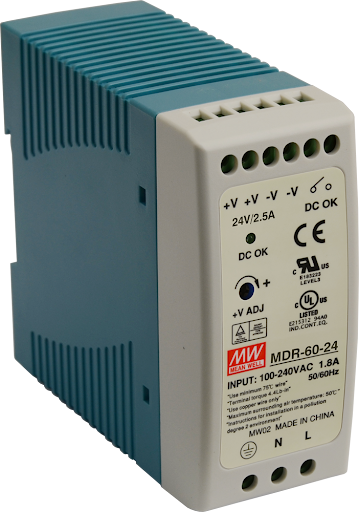
\includegraphics[width=2.2cm]{Images/Chap2/MeanWell.png} & Provides stable 24V DC power to the PLC, sensors, contactors, and other control components. \\
        \hline
        \textbf{Power Supply MDR-60-5} & Mean Well &
        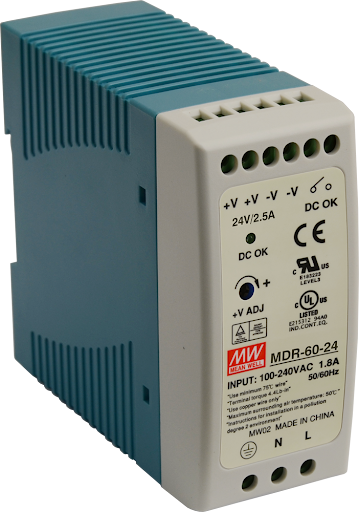
\includegraphics[width=2.2cm]{Images/Chap2/MeanWell.png} & Provides stable 5V DC power to Power the Raspberry Pi. \\
        \hline
    \end{tabularx}
\end{table}

\subsubsection{Control components}
This section details the primary control and logic components of the electrical system. The components used are listed in Table \ref{tab:control_components}.
\begin{table}[H]
    \centering
    \caption{Control Components Used in the Electrical Cabinet}
    \label{tab:control_components}
    \begin{tabularx}{\textwidth}{| >{\raggedright}p{0.3\textwidth} | >{\centering}m{0.2\textwidth} | >{\centering\arraybackslash}m{2.8cm} | X |}
        \hline
        \textbf{Name and Description} & \textbf{Brand} & \textbf{Figure} & \textbf{Function} \\
        \hline
        \textbf{S7-1200 PLC (CPU 1214C)} & Siemens &
        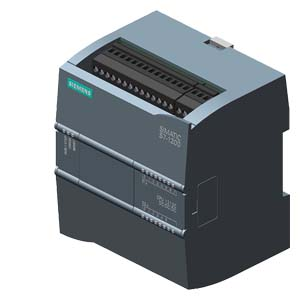
\includegraphics[width=2.5cm]{Images/Chap2/PLC.jpg} & Controls the system logic, managing inputs/outputs, safety signals, and emergency stops. \\
        \hline
        \textbf{ Contactor 
        -TeSys LC1-D - 3 poles - AC-3 440V 18 A - coil 24 V AC} & Schneider Electric &
        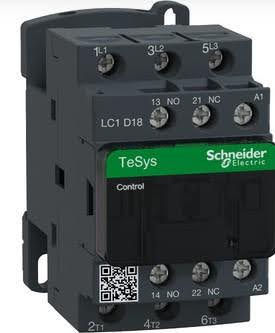
\includegraphics[width=2.5cm]{Images/Chap2/TeSys LC1.jpg} & Used to switch AC loads like conveyor motors. It acts as a safety device, cutting power when the emergency button is pressed. \\
        \hline
        \textbf{Key Selector Switch - Harmony XB4 - 3131A key switch - Ø22 - 2 pos fixed - spring return G } & Schneider Electric &
        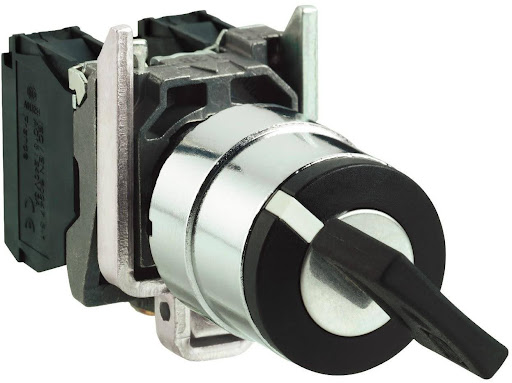
\includegraphics[width=2.5cm]{Images/Chap2/Harmony XB4.jpg} & Allows the operator to switch the main power on or off. \\
        \hline
        \textbf{LED Indicator Light - Harmony XB4 - LED indicator - Ø22 - red - 230V} & Schneider Electric &
        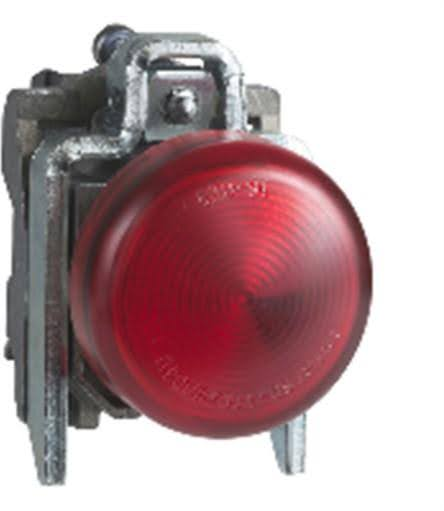
\includegraphics[width=2.5cm]{Images/Chap2/voyant lumineux DEL.jpg} & Indicates system power status. \\
        \hline
        \textbf{Green Push Button - Harmony XB4 - impulse push button - Ø22 - green - 1F} & Schneider Electric &
        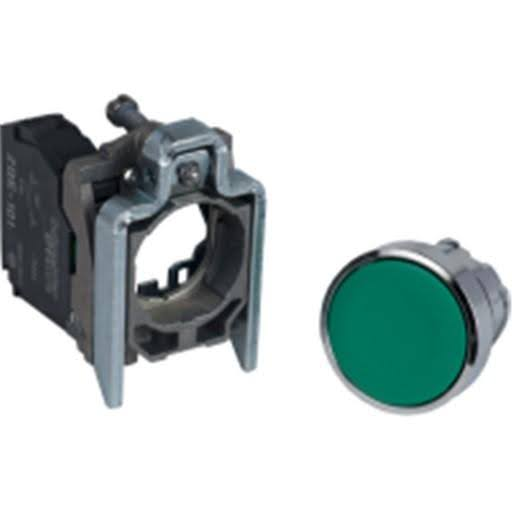
\includegraphics[width=2.5cm]{Images/Chap2/bouton poussoir à impulsion.jpg} & Used to start the system. \\
        \hline
        \textbf{Black Push Button - Harmony XB4 - impulse push button - Ø22 - black - 1F} & Schneider Electric &
        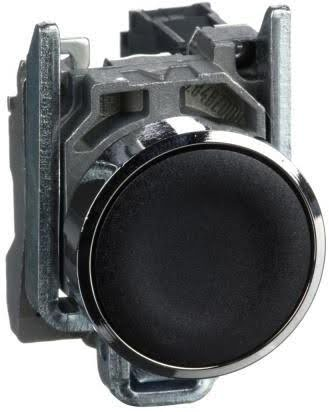
\includegraphics[width=2.5cm]{Images/Chap2/Harmony XB4 - bouton poussoir à impulsio.jpg} & Used to stop or reset the system. \\
        \hline
        \textbf{Emergency Stop Push Button - XB4 emergency stop push button - Harmony- Ø 22mm - red - push/pull} & Schneider Electric &
        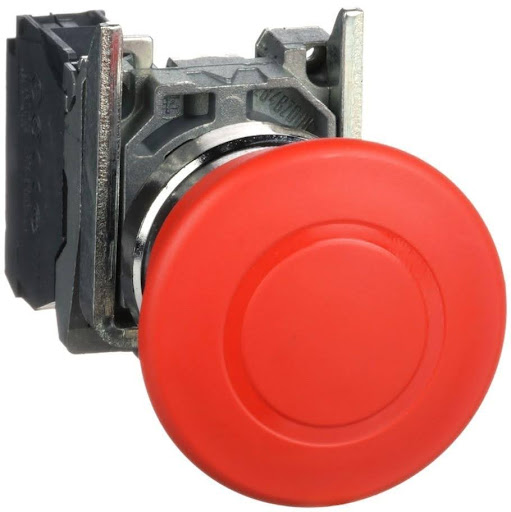
\includegraphics[width=2.5cm]{Images/Chap2/Harmony - bouton poussoir arrêt d'urgence XB4.jpg} & Used for emergency stops to immediately halt all system operations for safety. \\
        \hline
    \end{tabularx}
\end{table}





\subsubsection{Other components}
This section lists additional components and hardware essential for the electrical cabinet's structure and wiring. Table \ref{tab:other_components} provides a list of these components.
\begin{table}[H]
    \centering
    \caption{Other Components Used in the Electrical Cabinet}
    \label{tab:other_components}
    \begin{tabularx}{\textwidth}{| >{\raggedright}p{0.3\textwidth} | >{\centering}m{0.2\textwidth} | >{\centering\arraybackslash}m{2.5cm} | X |}
        \hline
        \textbf{Name and Description} & \textbf{Brand} & \textbf{Figure} & \textbf{Function} \\
        \hline
        \textbf{GT 80-40-25} & Schneider Electric &
        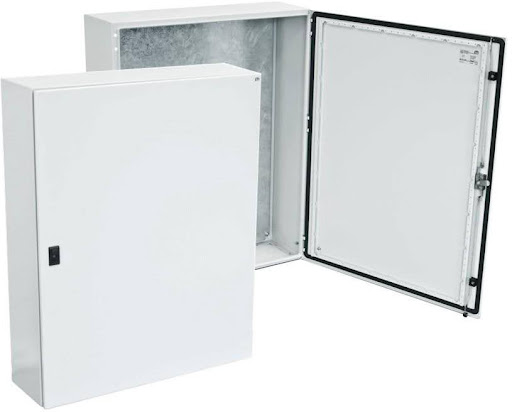
\includegraphics[width=2.5cm]{Images/Chap2/GT 80-40-25.jpg} & Protects electrical and electronic components from dust, moisture, and external impacts. \\
        \hline
        \textbf{Rittal Slotted Panel Trunking, W30 mm x} & Rittal &
        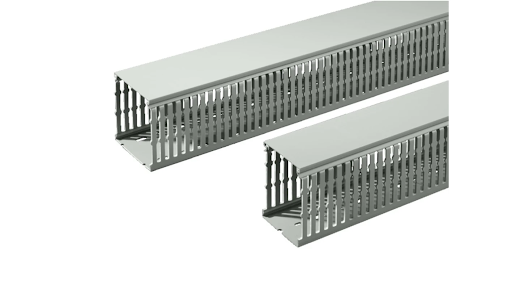
\includegraphics[width=2.5cm]{Images/Chap2/Rittal Slotted Panel Trunki.png} & Organizes and protects cables inside control panels. \\
        \hline
        \textbf{TERMINAL BLOCK WT 16 MM² WKN 16/U V0 GRIS} & Phoenix Contact &
        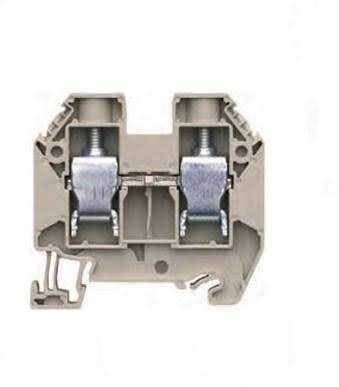
\includegraphics[width=2.5cm]{Images/Chap2/BORNIER.jpg} & Connects and distributes electrical wires safely. \\
        \hline
        \textbf{SZ Support rail to EN 60 715, version TH 35/15, L : 2000 mm} & Phoenix Contact &
        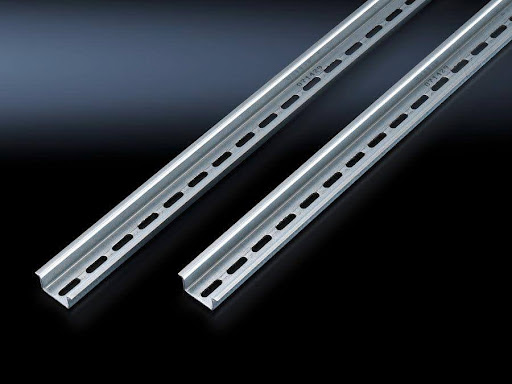
\includegraphics[width=2.5cm]{Images/Chap2/SZ Support rail.jpg} & For snap-mounting terminals or other components with a snap-in system to EN 60 715. \\
        \hline
        \textbf{DS-3E0505-O} & Hikvision &
        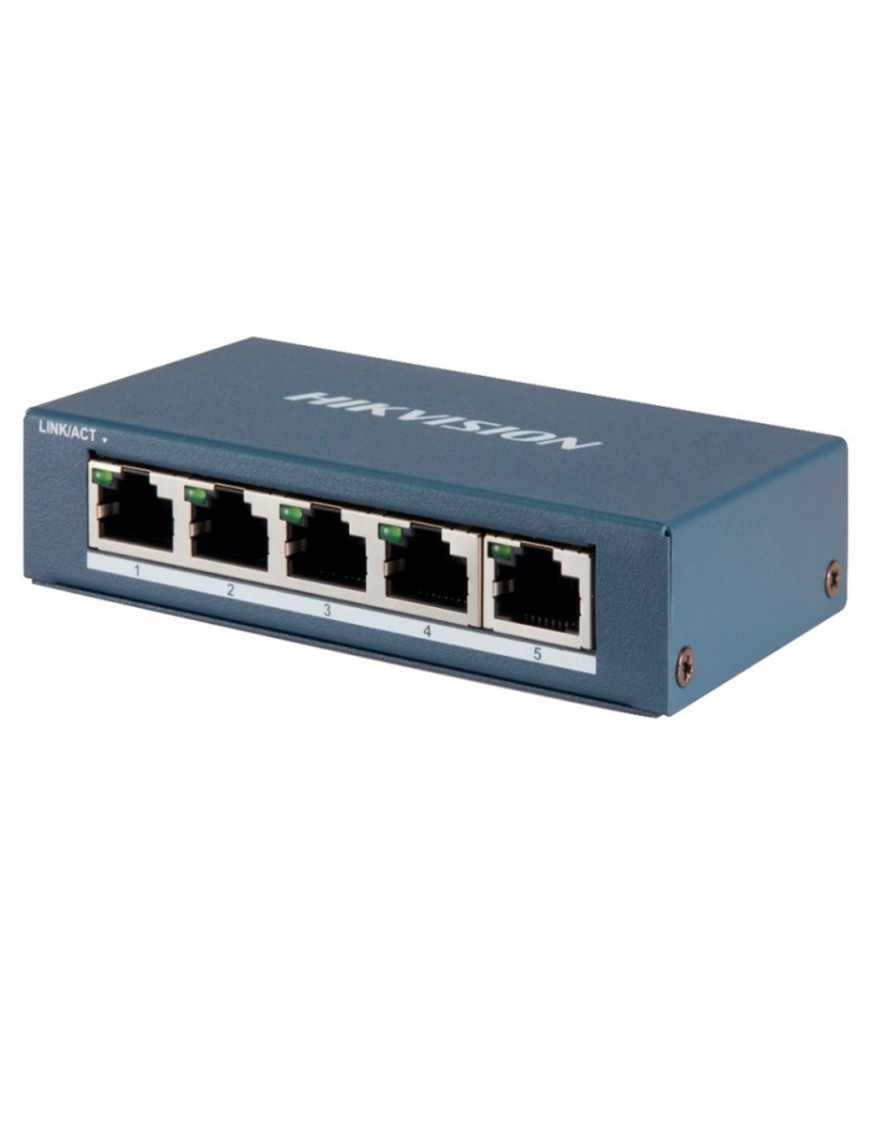
\includegraphics[width=2.5cm]{Images/Chap2/Switch-hikvision-5x-ports-gigabit-unmanaged-tunisie.jpg} & Provides 5 Gigabit RJ45 ports with 1000M network access. \\
        \hline
    \end{tabularx}
\end{table}




\subsubsection{2D and 3D Cabinet Layout}
The following diagrams, generated using E-Plan software, provide a detailed visual representation of the electrical cabinet's layout, as shown in Figure \ref{fig:eplan_layouts}. They illustrate the precise placement of components and the overall physical architecture, ensuring an organized and optimized setup for efficient operation and maintenance.

\begin{figure}[H]
    \centering
    \subfloat[Front door layout]{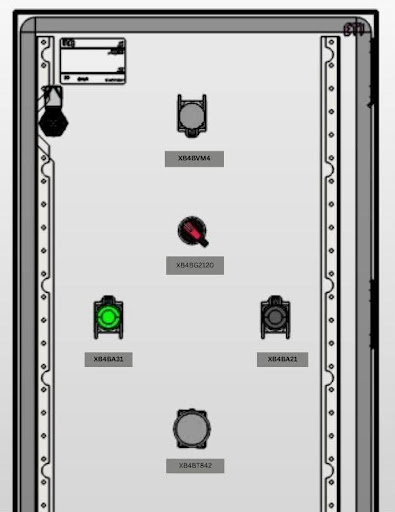
\includegraphics[width=0.3\textwidth]{Images/Chap2/front.jpg}\label{fig:front_door_layout}}
    \hfill % Adds spacing between the images
    \subfloat[Internal layout]{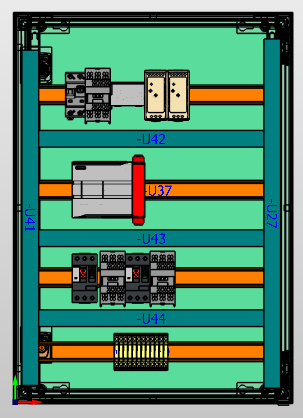
\includegraphics[width=0.28\textwidth]{Images/Chap2/inside.png}\label{fig:internal_layout}}
    \hfill % Adds spacing between the images
    \subfloat[3D View]{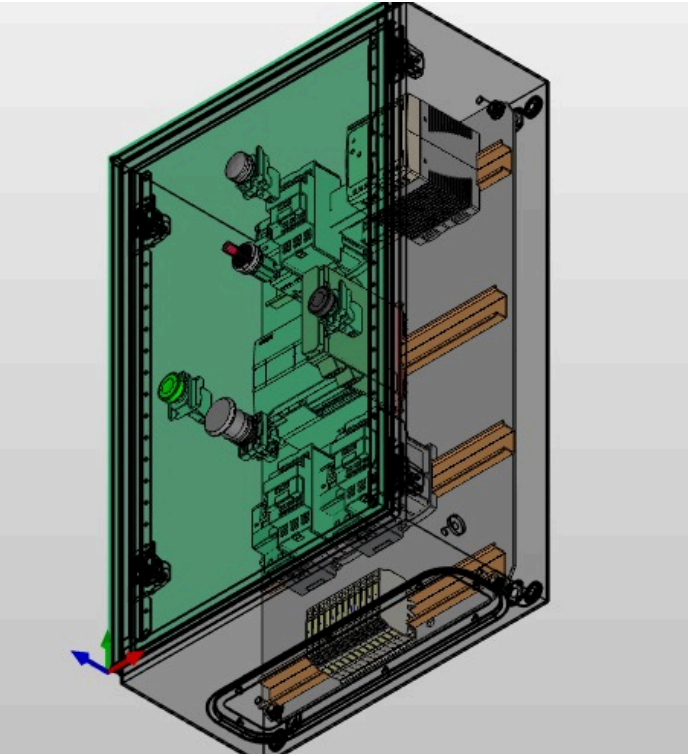
\includegraphics[width=0.3\textwidth]{Images/Chap2/3dlook.png}\label{fig:3d_layout}}
    \caption[E-Plan Electrical Cabinet Layouts]{E-Plan Electrical Cabinet Layouts}
    \label{fig:eplan_layouts}
\end{figure}

\subsection{Pneumatic Cabinet}
The pneumatic cabinet serves as the central hub for compressed air management and motion control within the automated system. It houses all main control components—including air preparation units, distribution manifolds, and solenoid valves—that are essential for the safe and precise operation of pneumatic actuators like cylinders and grippers. The cabinet ensures a clean and organized system, while also facilitating maintenance and future scalability for pneumatic circuits.

\subsubsection{Pneumatic Wiring Diagram}
To ensure the precise operation and sequencing of pneumatic actuators, a detailed wiring diagram was developed. This diagram, along with the components, which are exclusively sourced from Festo, illustrates the controlled flow of compressed air. The pneumatic circuit is presented in Annex \ref{fig:pneumatic_diagram}, which is accompanied by a detailed list of each numbered element, as shown in Table \ref{tab:pneumatic_components}, from the air preparation unit to the final actuators.



\begin{longtable}{|c|p{0.7\textwidth}|}
\caption{Pneumatic Components in the Wiring Diagram}
\label{tab:pneumatic_components}\\
\hline
\textbf{Designation} & \textbf{Description} \\
\hline
\endhead
1 & Parallel Cylinder for Gripper \\
\hline
2 & Guiding Cylinder \\
\hline
3 & Ejector Cylinder \\
\hline
4 & check Valve \\
\hline
5 & 5/3 Directional Valve \\
\hline
6 & 3/2 Directional Valve ( Closed Center ) \\
\hline
7 & Pressure Gauge \\
\hline
8 & Pressure Regulator \\
\hline
9 & flow control valve \\
\hline
10 & Air Treatment Unit \\
\hline
\end{longtable}


\subsubsection{Air Preparation Components}
This subsection details the components responsible for preparing and conditioning the compressed air supply before it is used by the system. The \textbf{FRL (Filter + Regulator + Lubricator) Unit} is a key component for this process, as it prepares the air supply by filtering out impurities, regulating the pressure to a constant level, and adding a small amount of lubricant to the air to ensure smooth operation of the pneumatic components. A visual representation of the FRL unit is provided in Figure \ref{fig:air_prep_components}.

\begin{figure}[H]
\centering
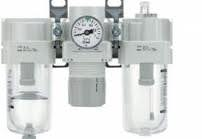
\includegraphics[width=0.4\textwidth]{Images/Chap2/FRLUnit.jpg}
\caption{FRL Unit (Filter + Regulator + Lubricator)}
\label{fig:air_prep_components}
\end{figure}










\subsubsection{Directional Control Valves}
These components are used to direct the flow of compressed air to the actuators, controlling their movement and position. The specific valves used in our system are detailed in Table \ref{tab:directional_valves}.

\begin{longtable}{|p{0.35\textwidth}|c|p{0.5\textwidth}|}
\caption{Directional Control Valves}
\label{tab:directional_valves}\\
\hline
\textbf{Name and Description} & \textbf{Figure} & \textbf{Function} \\
\hline
\endhead
\textbf{5/3 Directional Valve} &
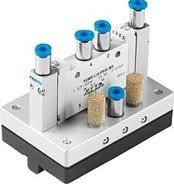
\includegraphics[width=2.5cm]{Images/Chap2/5-3Valve.jpg} & Directs air to cylinders. \\
\hline
\textbf{3/2 Directional Valve} &
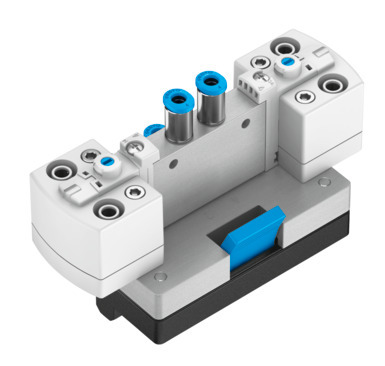
\includegraphics[width=2.5cm]{Images/Chap2/3-2Valve.jpg} & Directs air to cylinders. \\
\hline
\end{longtable}

\subsubsection{Flow and Pressure Control Components}
This section lists components that regulate the pressure and control the speed of air flow to ensure precise movement of the pneumatic actuators. The key components we integrated are shown in Table \ref{tab:flow_pressure_components}.

\begin{longtable}{|p{0.35\textwidth}|c|p{0.5\textwidth}|}
\caption{Flow and Pressure Control Components}
\label{tab:flow_pressure_components}\\
\hline
\textbf{Name and Description} & \textbf{Figure} & \textbf{Function} \\
\hline
\endhead
\textbf{Flow Regulator} &
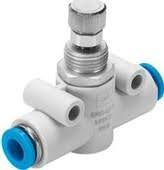
\includegraphics[width=2.5cm]{Images/Chap2/FlowRegulator.jpg} & Controls the air flow rate. \\
\hline
\textbf{Check Valve} &
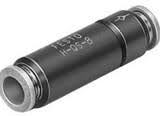
\includegraphics[width=2.5cm]{Images/Chap2/CheckValve.jpg} & Allows one-way airflow only. \\
\hline
\end{longtable}

\subsubsection{Distribution and Safety Components}
This section outlines the essential components for distributing air and ensuring the safety of the pneumatic system. A detailed list of these components is provided in Table \ref{tab:distribution_components}.

\begin{longtable}{|p{0.35\textwidth}|c|p{0.5\textwidth}|}
\caption{Distribution and Safety Components}
\label{tab:distribution_components}\\
\hline
\textbf{Name and Description} & \textbf{Figure} & \textbf{Function} \\
\hline
\endhead
\textbf{Pneumatic Manifold} &
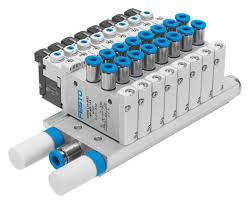
\includegraphics[width=2.5cm]{Images/Chap2/PneumaticManifold.jpg} & Provides a central point for air distribution and serves as a mounting block for multiple control valves, simplifying the circuit. \\
\hline
\textbf{Lockout Valve} &
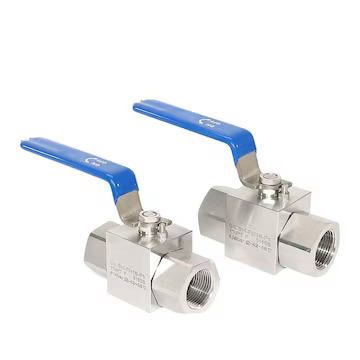
\includegraphics[width=2.5cm]{Images/Chap2/LockoutValve.jpg} & A manual shut-off valve that isolates the pneumatic system from the main air supply for safe maintenance and service. \\
\hline
\textbf{Pneumatic Tubing (4mm)} &
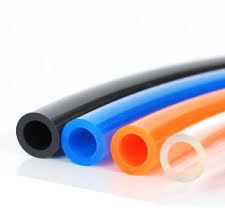
\includegraphics[width=2.5cm]{Images/Chap2/PneumaticTubing.jpg} & Flexible tubing used to create the physical connections for distributing compressed air between all components in the pneumatic circuit. \\
\hline
\end{longtable}







\subsection{Vision System}
The vision system provides the necessary intelligence for color-based classification. Its hardware is designed for reliability and cost-effectiveness in an industrial environment, with the components detailed in Table \ref{tab:vision_hardware}.

\begin{table}[H]
    \centering
    \caption{Vision System Hardware Components}
    \label{tab:vision_hardware}
    \begin{tabularx}{\textwidth}{| >{\raggedright}p{0.4\textwidth} | >{\centering\arraybackslash}m{3.5cm} | X |}
        \hline
        \textbf{Name and Description} & \textbf{Figure} & \textbf{Function} \\
        \hline
        \textbf{Raspberry Pi 4 Model B} &
        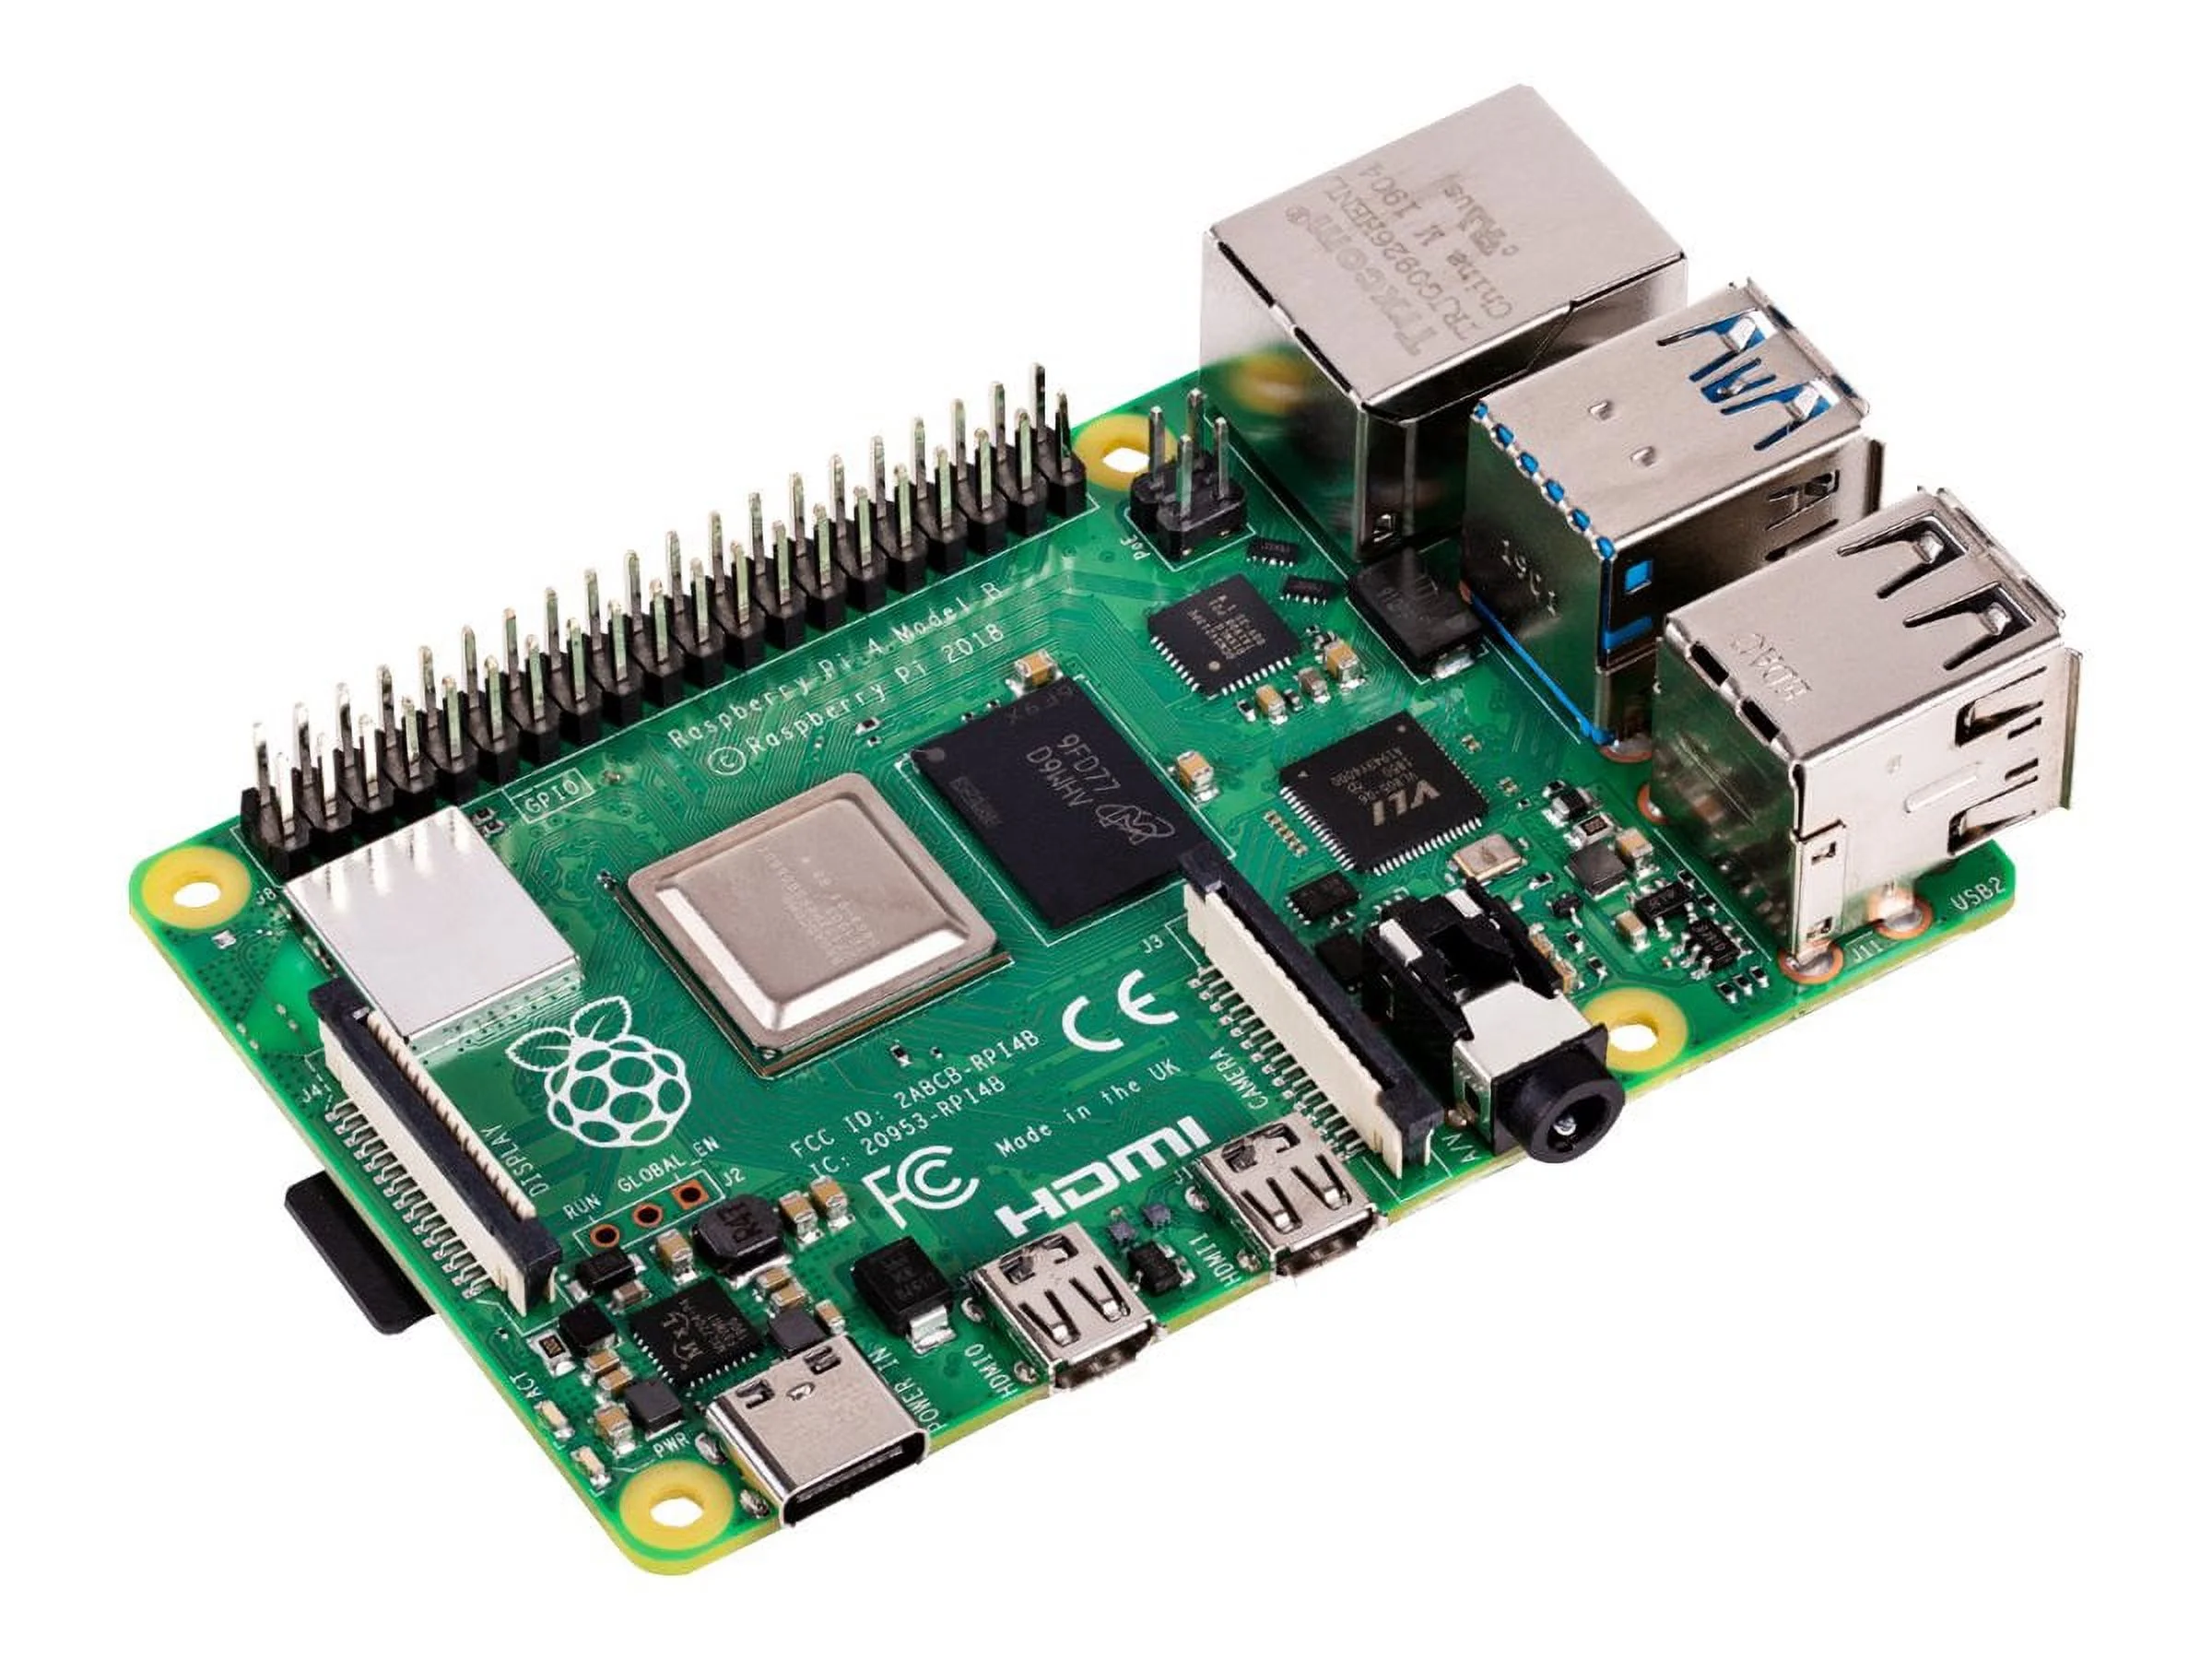
\includegraphics[width=3cm]{Images/Chap2/RaspberryPi4.png} & Serves as the central processing unit for image acquisition and color detection. \\
        \hline
        \textbf{Raspberry Pi Camera Module V2} &
        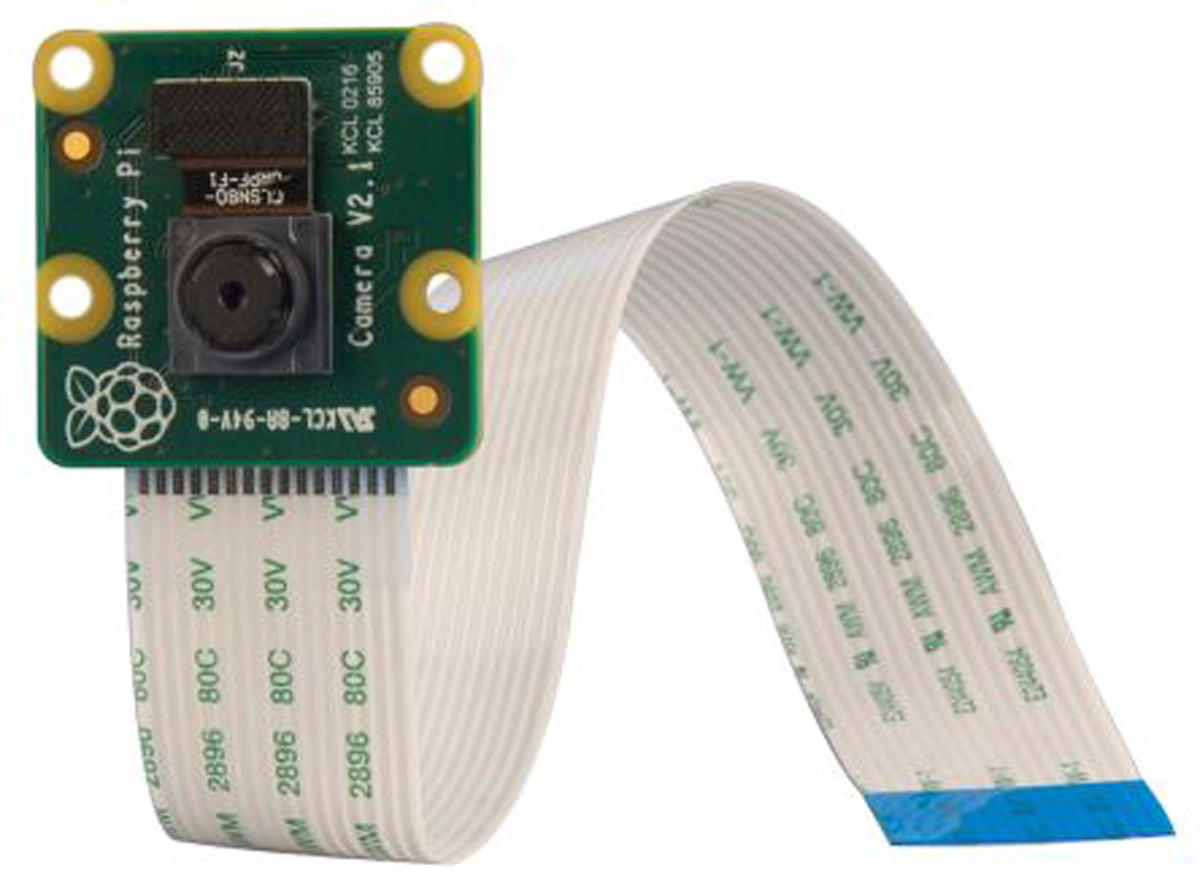
\includegraphics[width=3cm]{Images/Chap2/PiCameraV2.jpg} & An 8-megapixel camera that captures high-quality images with accurate color reproduction. \\
        \hline
        \textbf{Raspberry Pi Case with Fan} &
        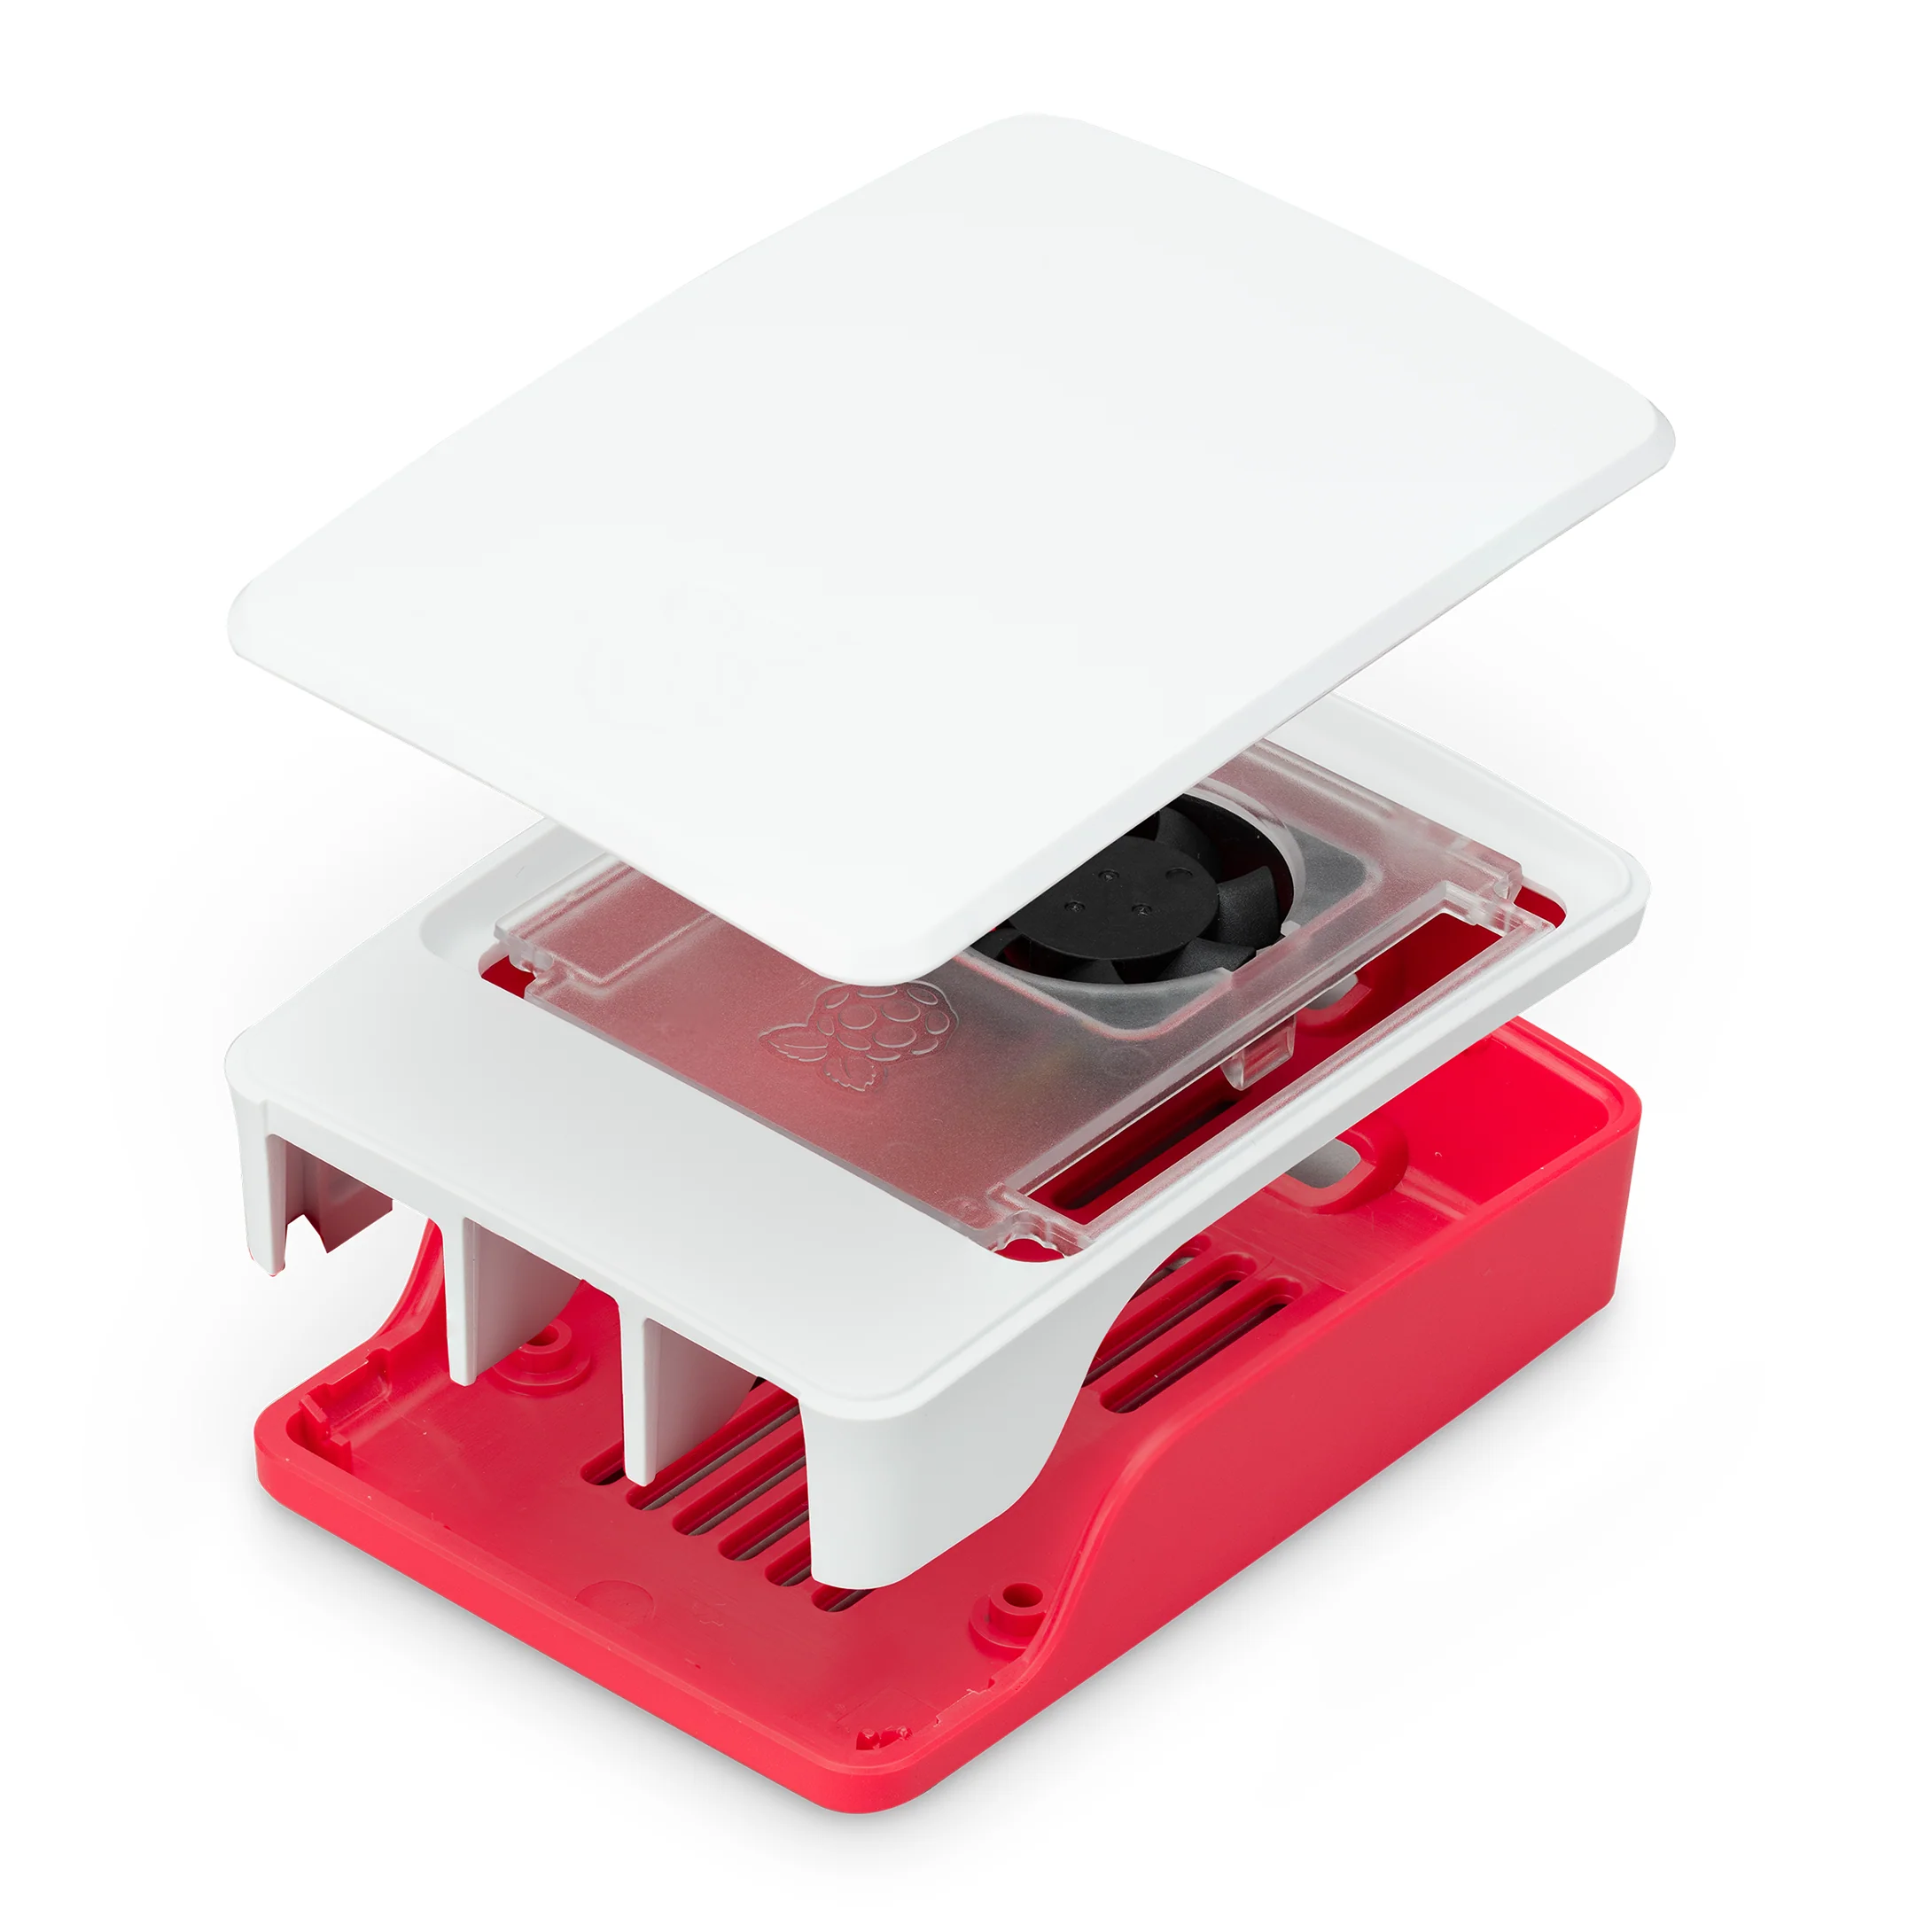
\includegraphics[width=3cm]{Images/Chap2/PiCaseFan.png} & A protective enclosure with an integrated fan to ensure stable performance. \\
        \hline
    \end{tabularx}
\end{table}
\section{Software Architecture}
The software architecture of the robotic sorting cell is built on a suite of specialized tools that integrate hardware control, design, simulation, and visualization. This approach ensures a streamlined workflow from conceptualization to implementation, with each software playing a distinct and crucial role.

\subsection{TIA Portal}
TIA Portal is a powerful and integrated software suite from Siemens that provides a single, unified environment for all automation tasks \hyperref[sec:bibliography]{[6]}. Its primary strength lies in its ability to centralize multiple engineering disciplines, including hardware configuration, PLC programming, and HMI design, into one platform. This integration was a key factor in its selection for this project, as it simplified the workflow, ensured data consistency across all components, and significantly reduced development time. The TIA Portal logo is shown in Figure \ref{fig:TIA_logo}.
\begin{figure}[H]
    \centering
    
\includegraphics[width=0.15\textwidth]{Images/Chap2/TIAPortal_logo.png}
    \caption{TIA Portal Logo}
    \label{fig:TIA_logo}
\end{figure}
\subsubsection{Key Advantages and Features}
The decision to use TIA Portal was driven by its numerous advantages that streamlined the development and commissioning of the automated sorting cell. The most significant benefits are outlined below:
\begin{itemize}
\item Integrated Engineering Environment: TIA Portal provides a single software platform for all automation tasks. This allows the entire project—from hardware setup and PLC logic to HMI design—to be managed within a unified environment, which eliminates the need for multiple software packages and ensures data consistency across all components;
\item Comprehensive Diagnostics and Troubleshooting: The software offers a powerful suite of diagnostic tools that provide real-time monitoring and fault analysis. This includes online functions to observe variable values, trace signal states, and identify network communication issues, which is critical for efficient debugging and commissioning;
\item Scalability and Reusability: TIA Portal's architecture is highly scalable, supporting a wide range of Siemens hardware, from small, modular PLCs to powerful, high-performance controllers. This flexibility allows for the easy expansion of a project;
\item Integrated Simulation: The platform provides a seamless connection to simulation software, such as S7-PLCSIM Advanced. This capability allows for virtual commissioning and testing of the control logic without physical hardware, significantly reducing development time and minimizing risks before deployment.
\end{itemize}

\subsubsection{Programming Languages and Communication Protocols}
TIA Portal supports a variety of programming languages that comply with the IEC 61131-3 standard, offering flexibility to developers. For this project, the primary languages used were Ladder Diagram and Structured Control Language. The supported languages include:
\begin{itemize}
\item Ladder Diagram (LAD): A graphical language that uses relay logic symbols, ideal for simple and sequential control;
\item Function Block Diagram (FBD): A graphical language that represents logic using interconnected function blocks;
\item Structured Control Language (SCL): A high-level, text-based language similar to Pascal, used for complex algorithms and data handling;
\item Statement List (STL): A low-level, text-based assembly-like language;
\item Sequential Function Chart (SFC): A graphical language used to model sequential processes.
\end{itemize}
In terms of communication, TIA Portal leverages a wide range of industry-standard protocols, including PROFINET, PROFIBUS, AS-Interface, and Ethernet/IP. While the platform supports this diverse array of communication standards, the primary protocol used for this project was PROFINET, a variant of industrial Ethernet, which enabled high-speed data exchange between the PLC, HMI, and other network devices.

\subsection{S7-PLCSIM Advanced V5.0}
S7-PLCSIM Advanced V5.0 is a powerful simulation tool that was used for virtual commissioning of the PLC program. It creates a virtual PLC that runs the exact same code as the physical hardware, allowing for comprehensive debugging and testing of the control logic without needing the real equipment. The S7-PLCSIM Advanced V5.0 logo is displayed in Figure \ref{fig:PLCSIM_logo}. This was particularly useful for verifying the complex state transitions of the GRAFCET sequence, as well as testing the synchronization between the virtual PLC and the robot's movements, saving significant time and resources during development. Annex \ref{fig:PLCSIM_workspace} shows the S7-PLCSIM Advanced Workspace for virtual commissioning.
\begin{figure}[H]
    \centering
    
\includegraphics[width=0.15\textwidth]{Images/Chap2/S7PLCSIMAdvanced_logo.jpg}
    \caption{S7-PLCSIM Advanced V5.0 Logo}
    \label{fig:PLCSIM_logo}
\end{figure}





\subsection{EPLAN}
EPLAN is an industry-standard software for creating professional electrical wiring diagrams and cabinet layouts. The EPLAN logo is presented in Figure \ref{fig:EPLAN_logo}. For this project, it was instrumental in designing the electrical schematics of the control cabinet and the pneumatic diagram. The use of EPLAN ensured that all wiring was logically organized, correctly documented, and compliant with safety standards. It also provided the necessary documentation for future maintenance and troubleshooting. The EPLAN workspace is shown in Annex \ref{fig:EPLAN_workspace}.
\begin{figure}[H]
    \centering
    
\includegraphics[width=0.2\textwidth]{Images/Chap2/EPLAN_logo.png}
    \caption{EPLAN Logo}
    \label{fig:EPLAN_logo}
\end{figure}


\subsection{Blender}
Blender is a versatile 3D computer graphics software that was used to develop a virtual model of the entire sorting cell\hyperref[sec:bibliography]{[7]}. The Blender logo is shown in Figure \ref{fig:Blender_logo}. This 3D model was crucial for visualizing the physical layout, optimizing the placement of the robot and conveyors, and simulating robot movements. The simulations in Blender were essential for verifying that the robot's reach was sufficient and that its motion paths were collision-free before any physical assembly took place, thereby mitigating potential design errors. The Blender workspace is shown in Annex \ref{fig:Blender_workspace}.
\begin{figure}[H]
    \centering
    
\includegraphics[width=0.2\textwidth]{Images/Chap2/Blender_logo.png}
    \caption{Blender Logo}
    \label{fig:Blender_logo}
\end{figure}


\subsection{WinCC Unified}
The HMI for the robotic sorting cell was developed using WinCC Unified, a powerful and modern platform seamlessly integrated within the TIA Portal framework. This technology represents a significant evolution from traditional HMI systems, offering key advantages that enhance the project's overall functionality and versatility.

Unlike conventional HMI systems (such as WinCC Comfort/Advanced), which typically rely on dedicated hardware panels or require specific runtime software to be installed on each client PC, WinCC Unified leverages modern web technologies. The HMI's interface is hosted on a central server, allowing it to be accessed directly through any standard web browser on a variety of devices. This capability is crucial, as it provides remarkable flexibility and portability, making the solution particularly impressive for public demonstrations and events. Figure \ref{fig:wincc_unified} illustrates the multi-platform capabilities of WinCC Unified.
\begin{figure}[H]
\centering
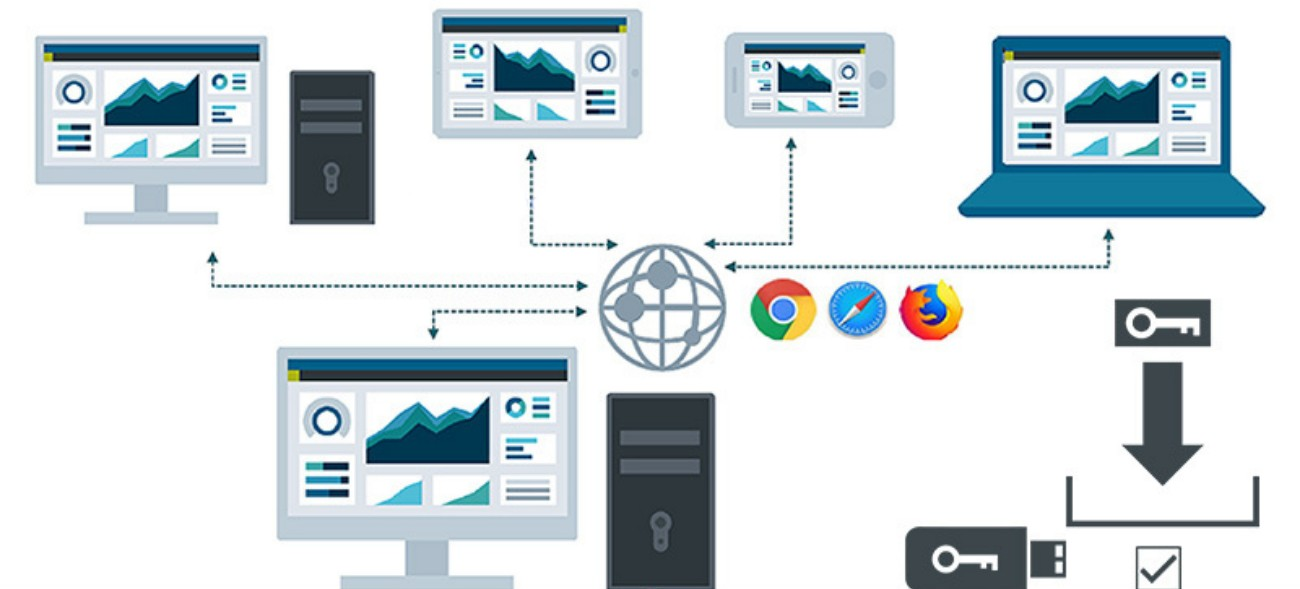
\includegraphics[width=0.7\textwidth]{Images/Chap3/unified.jpg}
\caption{WinCC Unified multi platform.}
\label{fig:wincc_unified}
\end{figure}
This web-based approach has several key benefits:
\begin{itemize}
\item Device Independence: The HMI can be viewed and controlled from a wide range of devices, including computers, tablets, and smartphones, without the need for additional client-side software.
\item Simplified Maintenance: Updates and changes to the HMI can be deployed centrally on the server, ensuring all clients are automatically using the latest version without individual updates.
\item Enhanced Accessibility: Operators and supervisors can monitor and interact with the system remotely from anywhere on the local network, improving operational oversight and responsiveness.
\end{itemize}

The project's HMI is deployed on a WinCC Unified Comfort Panel, but its browser-based design ensures that the interface is accessible from any client device, offering a scalable and future-proof solution.


\subsection{Python}
Python\hyperref[sec:bibliography]{[8]} is a high-level, interpreted programming language widely used in various applications, including computer vision, data analysis, and automation. Its simplicity and extensive libraries, such as \textbf{OpenCV}\hyperref[sec:bibliography]{[9]}, make it an ideal choice for the vision system in this project. Specifically, the Python script developed for this cell utilizes the OpenCV library for all image processing tasks.

\begin{figure}[H]
    \centering
    
\includegraphics[width=0.2\textwidth]{Images/Chap2/Python_logo.png}
    \caption{Python Logo.}
    \label{fig:Python_logo}
\end{figure}

The Python script is responsible for:
\begin{itemize}
    \item \textbf{Image Acquisition}:Capturing high-resolution images of the objects on the conveyor belt from the Raspberry Pi Camera Module;
    \item \textbf{Color Detection}: Analyzing the captured images to identify the color of each object using color space conversions and masking techniques;
    \item \textbf{Communication}: Sending the color information to the PLC via a TCP/IP or Ethernet connection, which then triggers the appropriate robot sequence for sorting.
\end{itemize}




\section{Conclusion}
This chapter provided a comprehensive overview of the automated sorting cell's foundational architecture, detailing its core hardware and software components. We explored the function of each element, from the central Programmable Logic Controller (PLC) and the Human-Machine Interface (HMI) to the KUKA robotic arm and the vision system. The discussion also covered the physical and logical cabinet layouts, establishing a robust framework for the system's safe and efficient operation. This thorough understanding of each component's role and its integration into the overall design is crucial for the successful implementation of the control logic detailed in the following chapters.









